%-----------------------------------------------------------------------------%
%                                                                             %
%    K A P I T E L   4                                                        %
%                                                                             %
%-----------------------------------------------------------------------------%

\chapter{Bipedal Walking Variants}\label{c4}
This chapter studies the proposed motion planning approach for bipedal walking gaits of the full-size humanoid RH5. It starts by describing the individual building blocks of the optimization problem, then discusses the simulation results obtained for increasing gait dynamics and finally provides an evaluation of the contact stability of the dynamic motions.

\section{Formulation of the Optimization Problem}\label{sec:BipedFormulation}
This section gives information about the adopted contact and impact modeling techniques and introduces the constraints used for generating physically consistent walking trajectories. The core formulation is based on the legged gaits described in \cite{mastalli20crocoddyl} but contains various improvements necessary for application on real robots. All motions presented in this chapter are solved for a predefined sequence of contacts and step timings. 
Recapitulating \cref{sec:TheoryDDP}, we formulate the optimization problem as
\begin{equation}\label{eqn:optimizationProblem}
\myM{X}^*,\myM{U}^*= 
\arg\min_{\mathbf{X},\mathbf{U}} l_N(x_N)+\sum_{k=0}^{N-1} \int_{t_k}^{t_k+\Delta t} l(\mathbf{x},\mathbf{u})dt. 
\end{equation}

\subsection{Contact and Impact Modeling}
During a walking motion, the body is always in contact with the ground either in single support, or in double support. In \cref{sec:TheoryConstrainedDDP} we have discovered, how rigid contacts can be expressed as a kinematic constraint on the \gls{EoM} (see \cref{eqn:unconstrainedDynamics}). 
Analogously, one can describe the impulse dynamics
\footnote{Impulse dynamics account for the physical effects that occur at a switch from non-contact to contact condition \cite{featherstone2014rigid}.} 
of a multibody system as
\begin{equation}\label{eqn:ImpulseDynamics}
\left[\begin{matrix}\myM{M} & \myM{J}^{\top}_c \\{\myM{J}_{c}} & \myM{0}\end{matrix}\right] \left[\begin{matrix} \myM{v}^+ \\ -\boldsymbol{\Lambda} \end{matrix}\right] = \left[\begin{matrix} \myM{M}\myM{v}^- \\ -e\myM{J}_c \myM{v}^-\end{matrix}\right],
\end{equation}
where $\boldsymbol{\Lambda}$ is the contact impulse, $\myM{v}^-$ and $\myM{v}^+$ are the generalized velocities before and after the impact and $e\in [0,1]$ is the restitution coefficient that accounts for the elasticity of the collision. For all motions, we use this impulse model to account for the infinitesimal short change in the contact situation. To improve the numerical integration stability, terms defined by Baumgarte Stabilization \cite{baumgarte1972stabilization} are used along with the rigid contact constraint described with \cref{eqn:gaussMinimization}. This numerical stabilization on the constraints can be expressed as:
\begin{equation}\label{eqn:BaumgarteStabilization}
a_0=a_{\lambda(c)}-\alpha M_{\lambda(c)}^{\text{ref}}\ominus M_{\lambda(c)}-\beta v_{\lambda(c)},
\end{equation}
where $a_0$ is the desired acceleration in the constrained space, $v_{\lambda(c)}, a_{\lambda(c)}$ are the spatial velocity and acceleration of the contact $\lambda(c)$, respectively, $M_{\lambda(c)}^{\text{ref}}\ominus M_{\lambda(c)}$ is the inverse composition between the reference contact placement and the current one \cite{mastalli20crocoddyl}. The PD gains $\alpha$ and $\beta$ enable an adequate numerical stabilization of the constraints depending on the dynamics of the movement.

\subsection{Robot Tasks}
Robot tasks, such as grasping and object or performing a step, are an essential goal of motion planning. As outlined in \cref{sec:TheoryConstrainedDDP}, these task-related constraints are considered in the optimization process as regulator functions. In the context of this thesis two tasks are of specific interest, namely the foot tracking and \gls{CoM} tracking. 

\paragraph{Foot Tracking Cost}
In order to perform a symmetric gait (see \cref{sec:TheoryBiped}), the design of dedicated foot trajectories is crucial. We use piecewise-linear functions to describe the swing foot reference trajectory. Deviation from this time-depended reference foot trajectory is highly penalized. The foot tracking cost can be formulated via the squared Euclidean norm (L2 norm) as
\begin{equation*} 
\Phi_{\text{foot}}=\mid\mid \myM{f}(t)-\myM{f}^{\text{ref}}(t)\mid\mid^2_2,
\end{equation*}
where $\myM{f}(t)$ is the actual \gls{CoM} position at time-step $t$ and $\myM{f}^\text{ref}(t)$ is the according reference. Start and end position as well as timings are predefined and combined with a desired step height to shape the desired foot trajectory. 

\paragraph{\Gls{CoM} Tracking Cost}
In bipedal locomotion, the three-dimensional position of the \gls{CoM} of the whole-body turned out to be crucial \cite{carpentier2017centre}. This is especially true for quasi-static motions, where the \gls{FCoM} is used as static stability margin as explained in \cref{sec:TheoryBiped}. Analogously to the foot cost, the \gls{CoM} tracking cost is formulated as
\begin{equation*} 
\Phi_{\text{CoM}}=\mid\mid \myM{c}(t)-\myM{c}^\text{ref}(t)\mid\mid^2_2.
\end{equation*}
In order to account for the static stability in these motions, we perform a dedicated shifting of the \gls{FCoM} to the foot center, before performing the swing-foot task. 
%Additionally, the \gls{CoM} is kept at a constant height to prevent unnecessary forces acting on the base of the body. 

\subsection{Inequality Constraints for Physical Consistency}
Essential demands on physically consistent motion planning are that (i) the robot limits (torque, joints) are considered and (ii) the generated trajectories are inherently balanced. To this end, we consider joint limits, friction cone and the novel \gls{CoP} bound as inequality constraints in our formulation, while torque constraints are covered in the algorithm itself.

\paragraph{Contact Stability Constraints}
As detailed in \cref{c3} with the concept of contact stability constrained \gls{DDP}, we constrain unilaterality, friction and \gls{CoP} for each foot in contact. For the sake of clarity, \cref{eqn:CoPCostComputation} is again recalled as 
\begin{equation*}
\Phi_{\text{CoP}}=
\begin{cases}
\quad\dfrac{1}{2}\myM{r}^T\myM{r} &\mid \text{lb} > \myM{r} > \text{ub} \\[10pt]
\quad 0 &\mid \text{lb} \leq \myM{r} \leq \text{ub},
\end{cases}
\end{equation*}
where the \gls{CoP} position is bound to lie inside the foot contact area by the lower and upper bounds $\text{lb}$ and $\text{ub}$, respectively.
In the same manner friction cone constraints along with the unilaterality are considered as
\begin{equation*}
\Phi_{\text{friction}}=
\begin{cases}
\quad\dfrac{1}{2}\myM{r}^T\myM{r} &\mid \text{lb} > \myM{r} > \text{ub} \\[10pt]
\quad 0 &\mid \text{lb} \leq \myM{r} \leq \text{ub},
\end{cases}
\end{equation*}
where $\text{lb}$ and $\text{ub}$ bound the resulting contact force to lie inside a four-sided polygonal approximation of the spatial friction cone \cite{kao2016contact}.

\paragraph{Joint Limits}
Physical boundaries of the joints must not be exceeded to avoid damage to the system. They are covered via a bounded quadratic activation as
\begin{equation*}
\Phi_{\text{joints}}=
\begin{cases}
\quad\dfrac{1}{2}\myM{r}^T\myM{r} &\mid \text{lb} > \myM{r} > \text{ub} \\[10pt]
\quad 0 &\mid \text{lb} \leq \myM{r} \leq \text{ub},
\end{cases}
\end{equation*}
where $\text{lb}$ and $\text{ub}$ correspond to the lower and upper bounds for joint position and velocities, respectively. 

\subsection{Further Regularization Terms}
Additional to the described constraints for tasks and physical consistency, we optimize for minimization of the torques and regularize the robot posture.
\paragraph{Torque Minimization}
In order to improve the energy efficiency of the motions and maintain a human-like torque at the joints \cite{kim1994modeling}, we minimize the joint torques for realistic dynamic movements via
\begin{equation*} 
\Phi_{\text{torque}}=\mid\mid \btau(t)\mid\mid^2_2.
\end{equation*}
\paragraph{Posture Regularization}
Finally, we deal with the redundancy of multi-body dynamics by applying a weighted least-squares cost function to regularize the state with respect to the nominal robot posture:
\begin{equation*} 
\Phi_{\text{posture}}=\mid\mid \myM{q}(t)-\myM{q}^\text{ref}(t)\mid\mid^2_2.
\end{equation*}


\section{Simulation Results for Increasing Gait Dynamics}\label{sec:BipedSimulation}
This section presents the simulation results for bipedal walking motions obtained by solving an optimization problem based on the described building blocks from the previous section. It studies both static and dynamic walking gaits, respectively.

\subsection{Static Walking}\label{subsec:StaticWalking}
The analysis of static walking gaits provides detailed insights on the optimization structure and allows a thorough experimental validation (see \cref{c7}).

Focus of investigation is a slow two step walking motion. We assume a quasi-static motion and hence deploy a static stability criterion as introduced in \cref{sec:TheoryStability} by following a dedicated \gls{FCoM} trajectory. To this end, the optimization problem is composed of a total of five locomotion phases visualized in \cref{fig:walkStatic_Snaps}. From (a) an initial pose, (b) shift the \gls{FCoM} above the \gls{LF}, (c) perform a right step, (d) shift the \gls{FCoM} above the \gls{RF}, (e) perform a left step and (f) shift the \gls{FCoM} to the half length of the line intersecting both feet center while returning to the initial pose.

Additionally, the \gls{CoM} is optimized for a constant height over the whole gait. \cref{tab:walkStatic} gives a compact overview of the desired gait characteristics and the applied constraints of the optimization. In order to comply with the quasi-static assumption, the motion is performed about a time horizon of 15 s with a total stride length of 20 cm a robot model with fixed arms. 
\begin{table}[t]
\centering
\caption[Static walking gait characteristics and optimization constraints]{Static walking gait characteristics and applied optimization constraints.}
\begin{tabular}{|ll|ll|}
\hline
\multicolumn{2}{|l|}{\textbf{Gait Characteristics}} & \multicolumn{2}{l|}{\textbf{Optimization Constraints}} \\ \hline
Step length:& 10 cm 	& Tasks: 			& $\Phi_{\text{foot}}$, $\Phi_{\text{CoM}}$\\ \hline
Step height:& 5 cm 	& Stability: 		& $\Phi_{\text{friction}}$\\ \hline
Time:& 3 s/phase 	& Limits: 			& $\Phi_{\text{joint}}$, torques \\ \hline
Step size:& 0.03 s	& Regularization: 	& $\Phi_{\text{posture}}$, $\Phi_{\text{torque}}$\\ \hline
\end{tabular}
\label{tab:walkStatic}
\end{table}

\begin{figure}
\begin{subfigure}{.16\textwidth}
	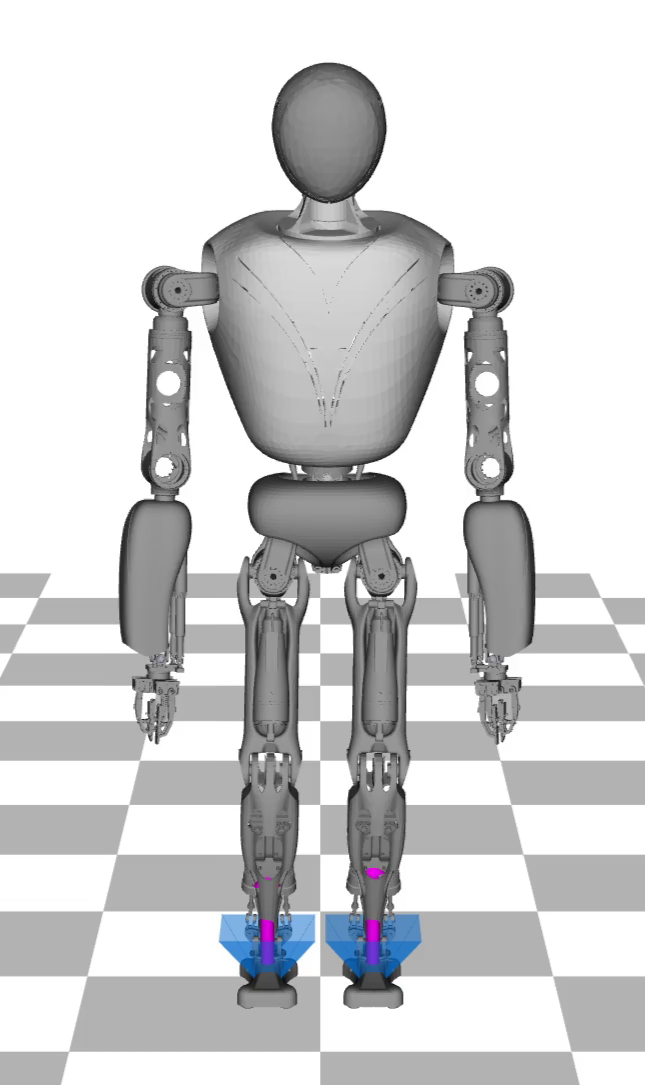
\includegraphics[width=.95\linewidth]{fig/walkStatic/snaps/1}
	\caption{}
\end{subfigure}%
\begin{subfigure}{.16\textwidth}
	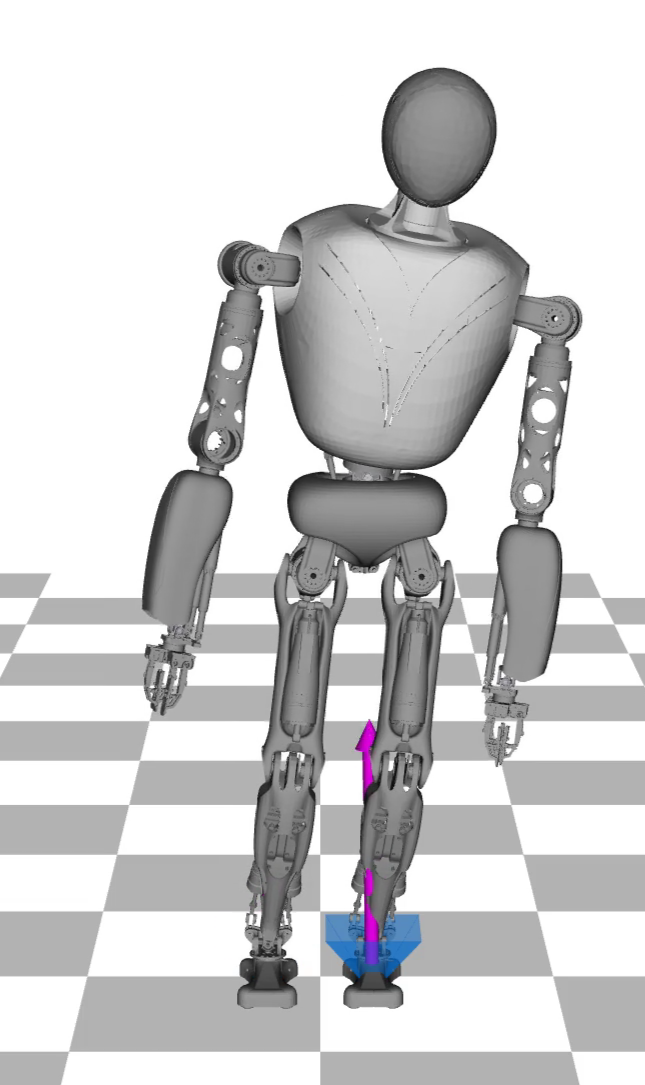
\includegraphics[width=.95\linewidth]{fig/walkStatic/snaps/2}
	\caption{}
\end{subfigure}%
\begin{subfigure}{.16\textwidth}
	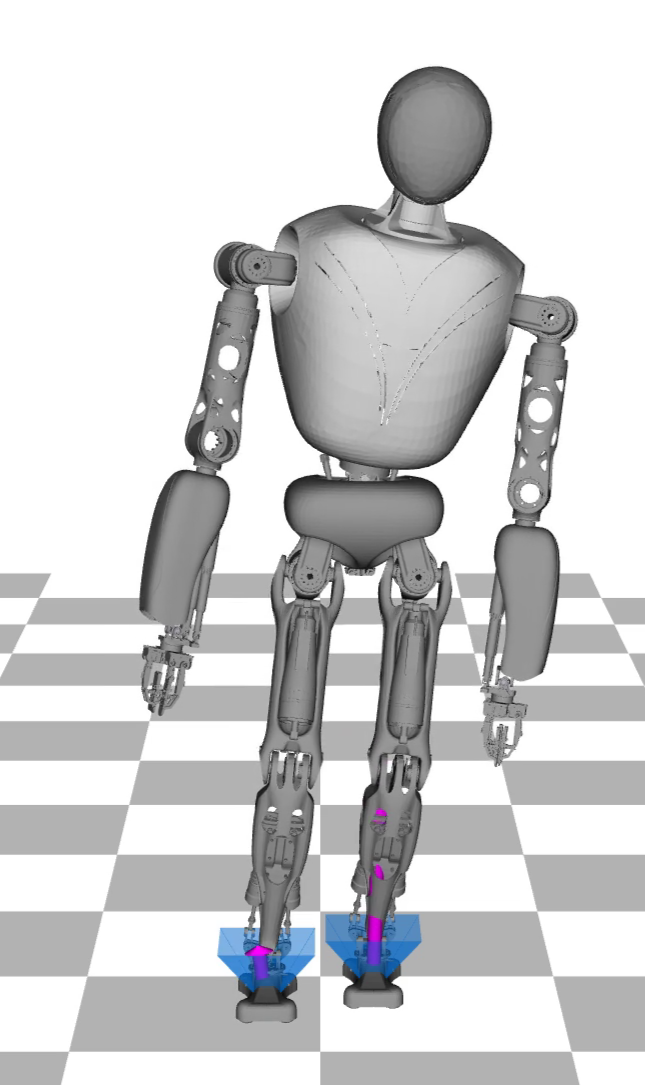
\includegraphics[width=.95\linewidth]{fig/walkStatic/snaps/4}
	\caption{}
\end{subfigure}%
\begin{subfigure}{.16\textwidth}
	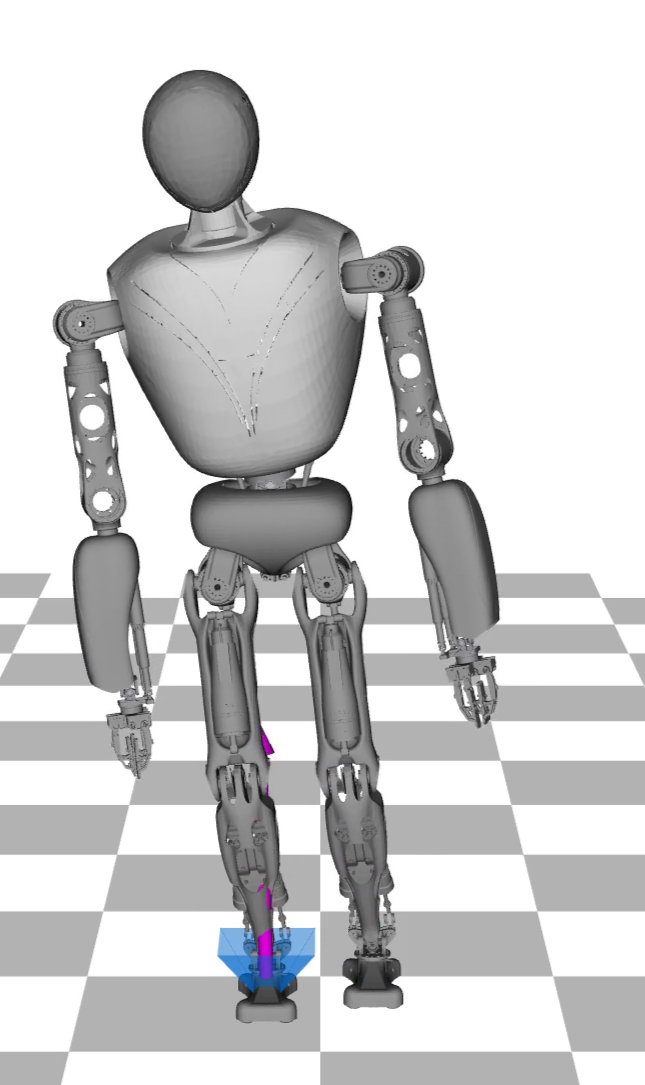
\includegraphics[width=.95\linewidth]{fig/walkStatic/snaps/6}
	\caption{}
\end{subfigure}%
\begin{subfigure}{.16\textwidth}
	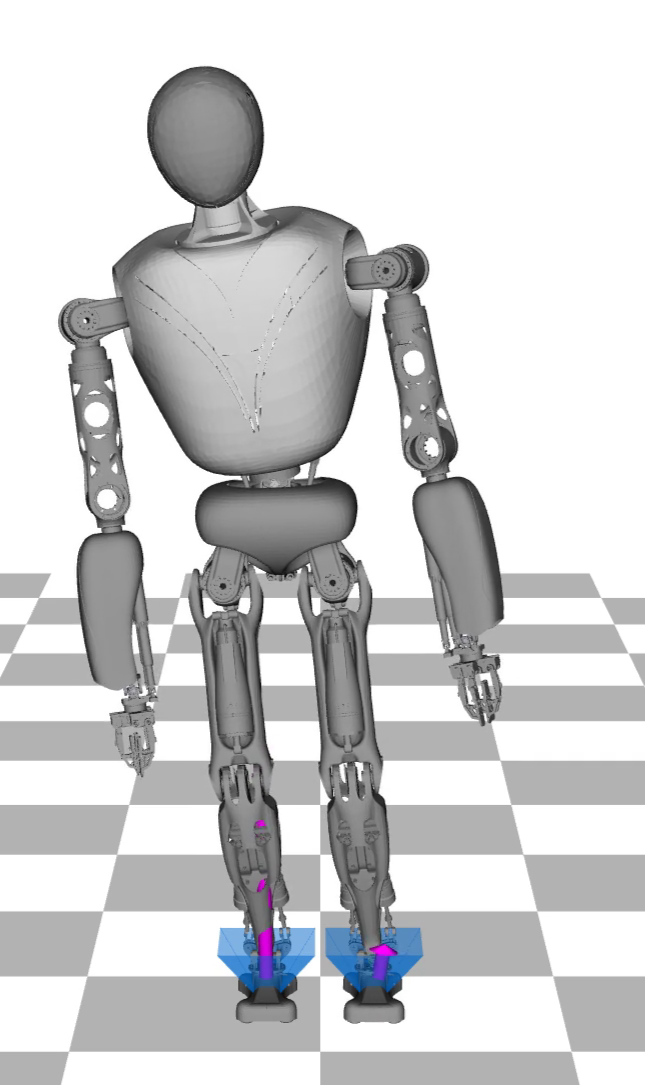
\includegraphics[width=.95\linewidth]{fig/walkStatic/snaps/8}
	\caption{}
\end{subfigure}%
\begin{subfigure}{.16\textwidth}
	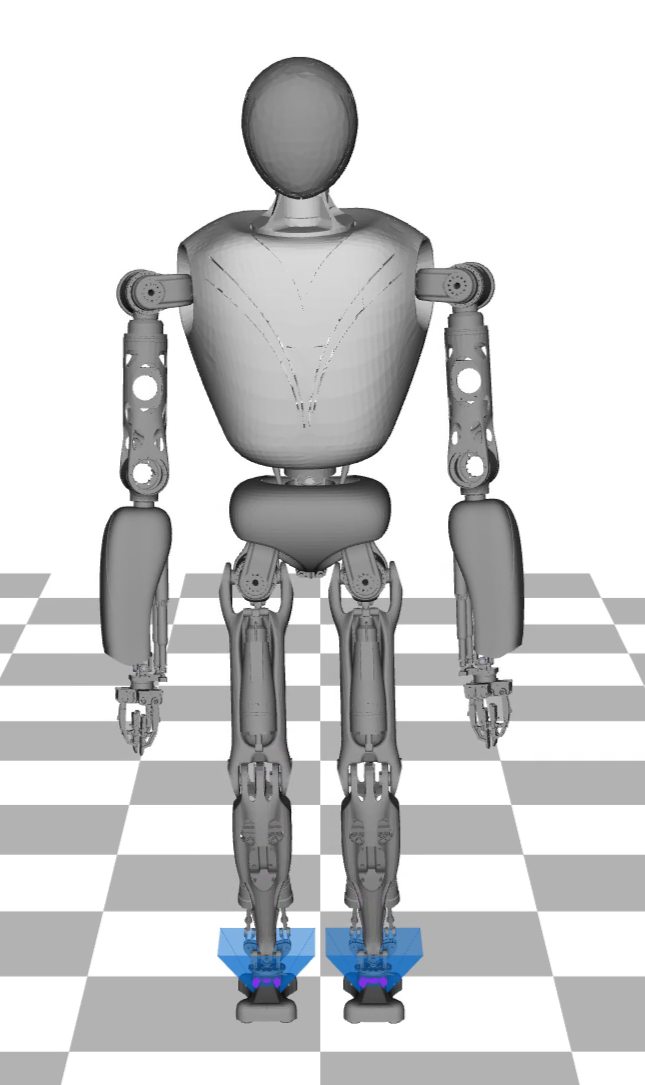
\includegraphics[width=.95\linewidth]{fig/walkStatic/snaps/9}
	\caption{}
\end{subfigure}
\caption[Static walking based on dedicated \gls{FCoM} shifting]{Static walking gait based on dedicated \gls{FCoM} motion, consisting of the locomotion phases (a) initial pose, (b) \gls{FCoM} shift above \gls{LF}, (c) right step, (d) \gls{FCoM} shift above \gls{RF}, (e) left step and (f) pose recovery. Significant lateral shifts of the \gls{FCoM} are required to establish the static stability. \href{https://github.com/julesser/ma-thesis-simulation-results/blob/master/HumanoidFixedArms/StaticWalking_NoCoPCost_ComHeightConstant/crocoddyl.mp4}{[Video]}}
\label{fig:walkStatic_Snaps}
\end{figure}

The results of the optimization problem \cref{eqn:optimizationProblem} are shown in \cref{fig:walkStatic_TaskSpace} and \cref{fig:walkStatic_JointState}.
\cref{fig:walkStatic_TaskSpace} presents the resulting base and end-effector trajectories. As becomes clear, the \gls{FCoM} tracking is sufficiently good and the \gls{CoM} height remains in a reasonable range of $\pm$ 1 cm. Equally, the desired foot trajectory is tracked with adequate accuracy. Also, the foot velocities are reasonable with a maximum velocity of 0.1 m/s at the impact. The pursued step height is not reached exactly but is about one centimeter less. This effect can be explained by the immediately reverse direction at the vertex of the piecewise-linear trajectory, which is smoothened by the solver.

\cref{fig:walkStatic_JointState} shows the resulting joint trajectories for the torso, \gls{LF} and \gls{RF}. Both the joint position limits and the maximum permissible joint speeds remain far below the limits due to the slow nature of the motion. Interestingly, the pursued \gls{FCoM} shifting turns out to be realized mostly based on a shift in the body roll activation rather than on a shift in the hips. Furthermore, it becomes evident that the posture regularization is effective since all joints end closely to the initial position.

\begin{figure}[h!]
\centering	
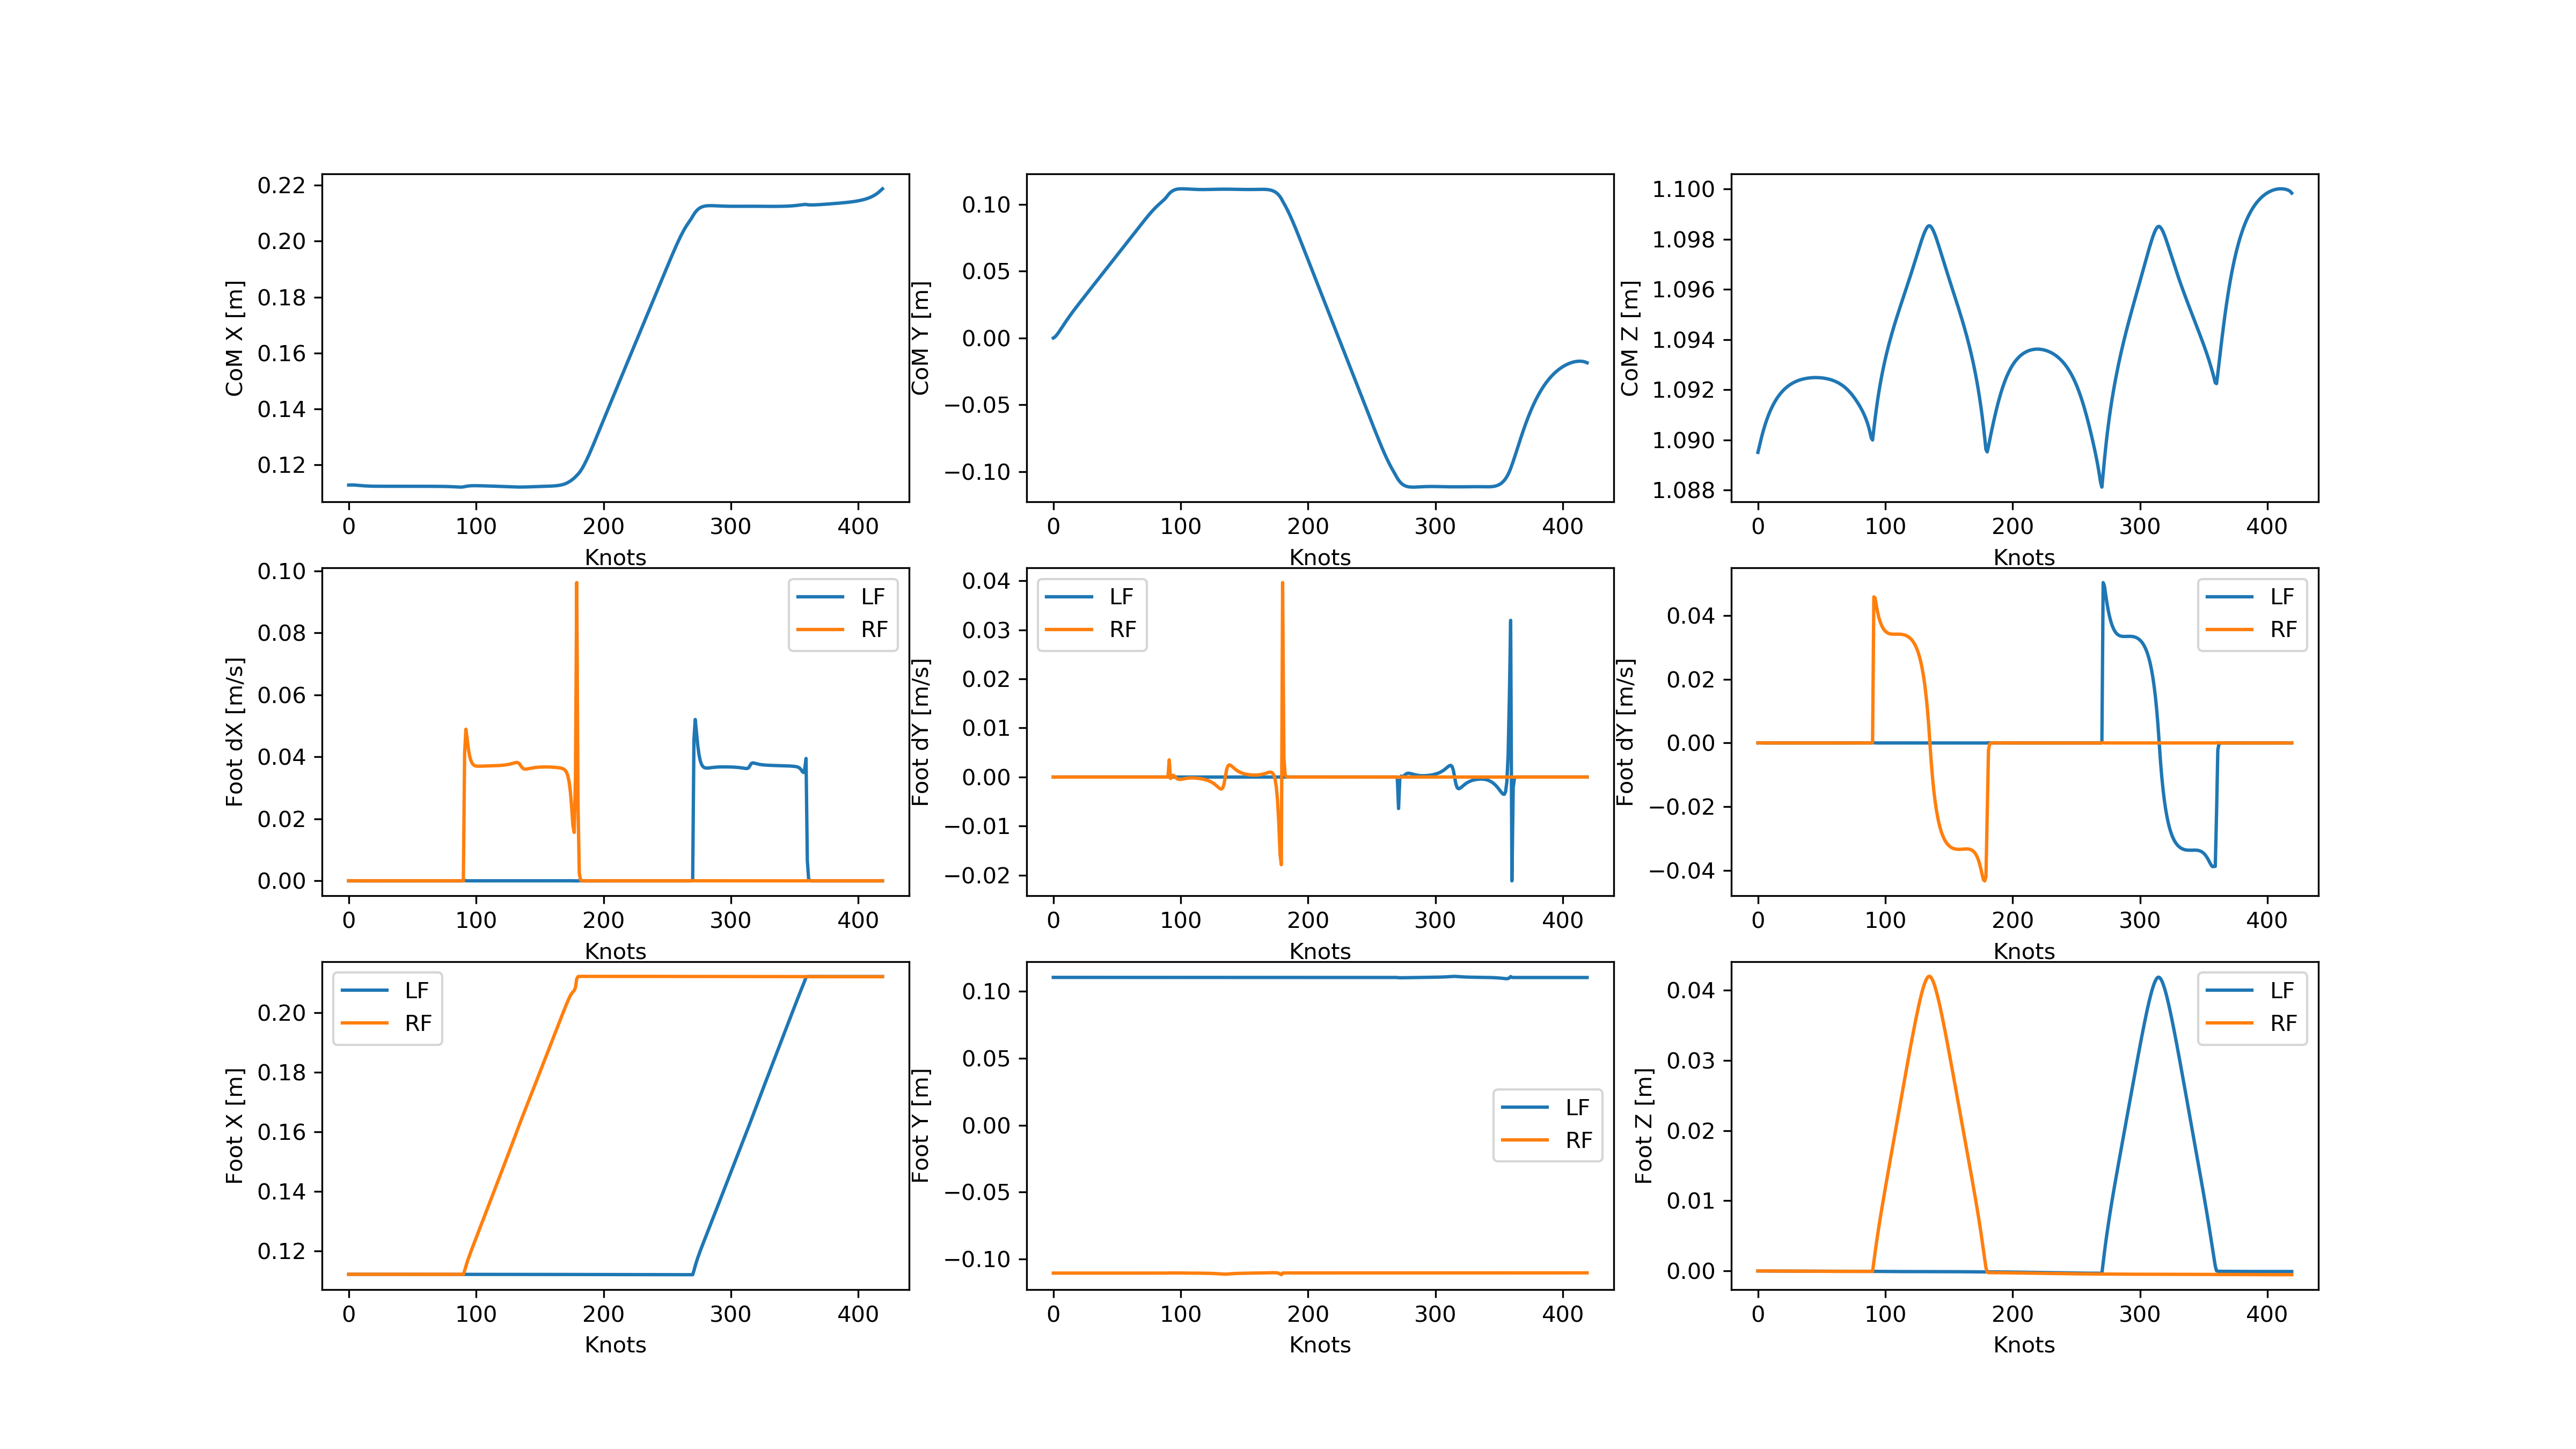
\includegraphics[width=1\textwidth]{fig/walkStatic/TaskSpace}
\caption[Static walking gait solution in task space]{Static walking gait solution in task space. Both the \gls{FCoM} task and the swing foot task are satisfied with acceptable accuracy.}
\label{fig:walkStatic_TaskSpace}
\end{figure} 

\begin{figure}[h!]
\centering	
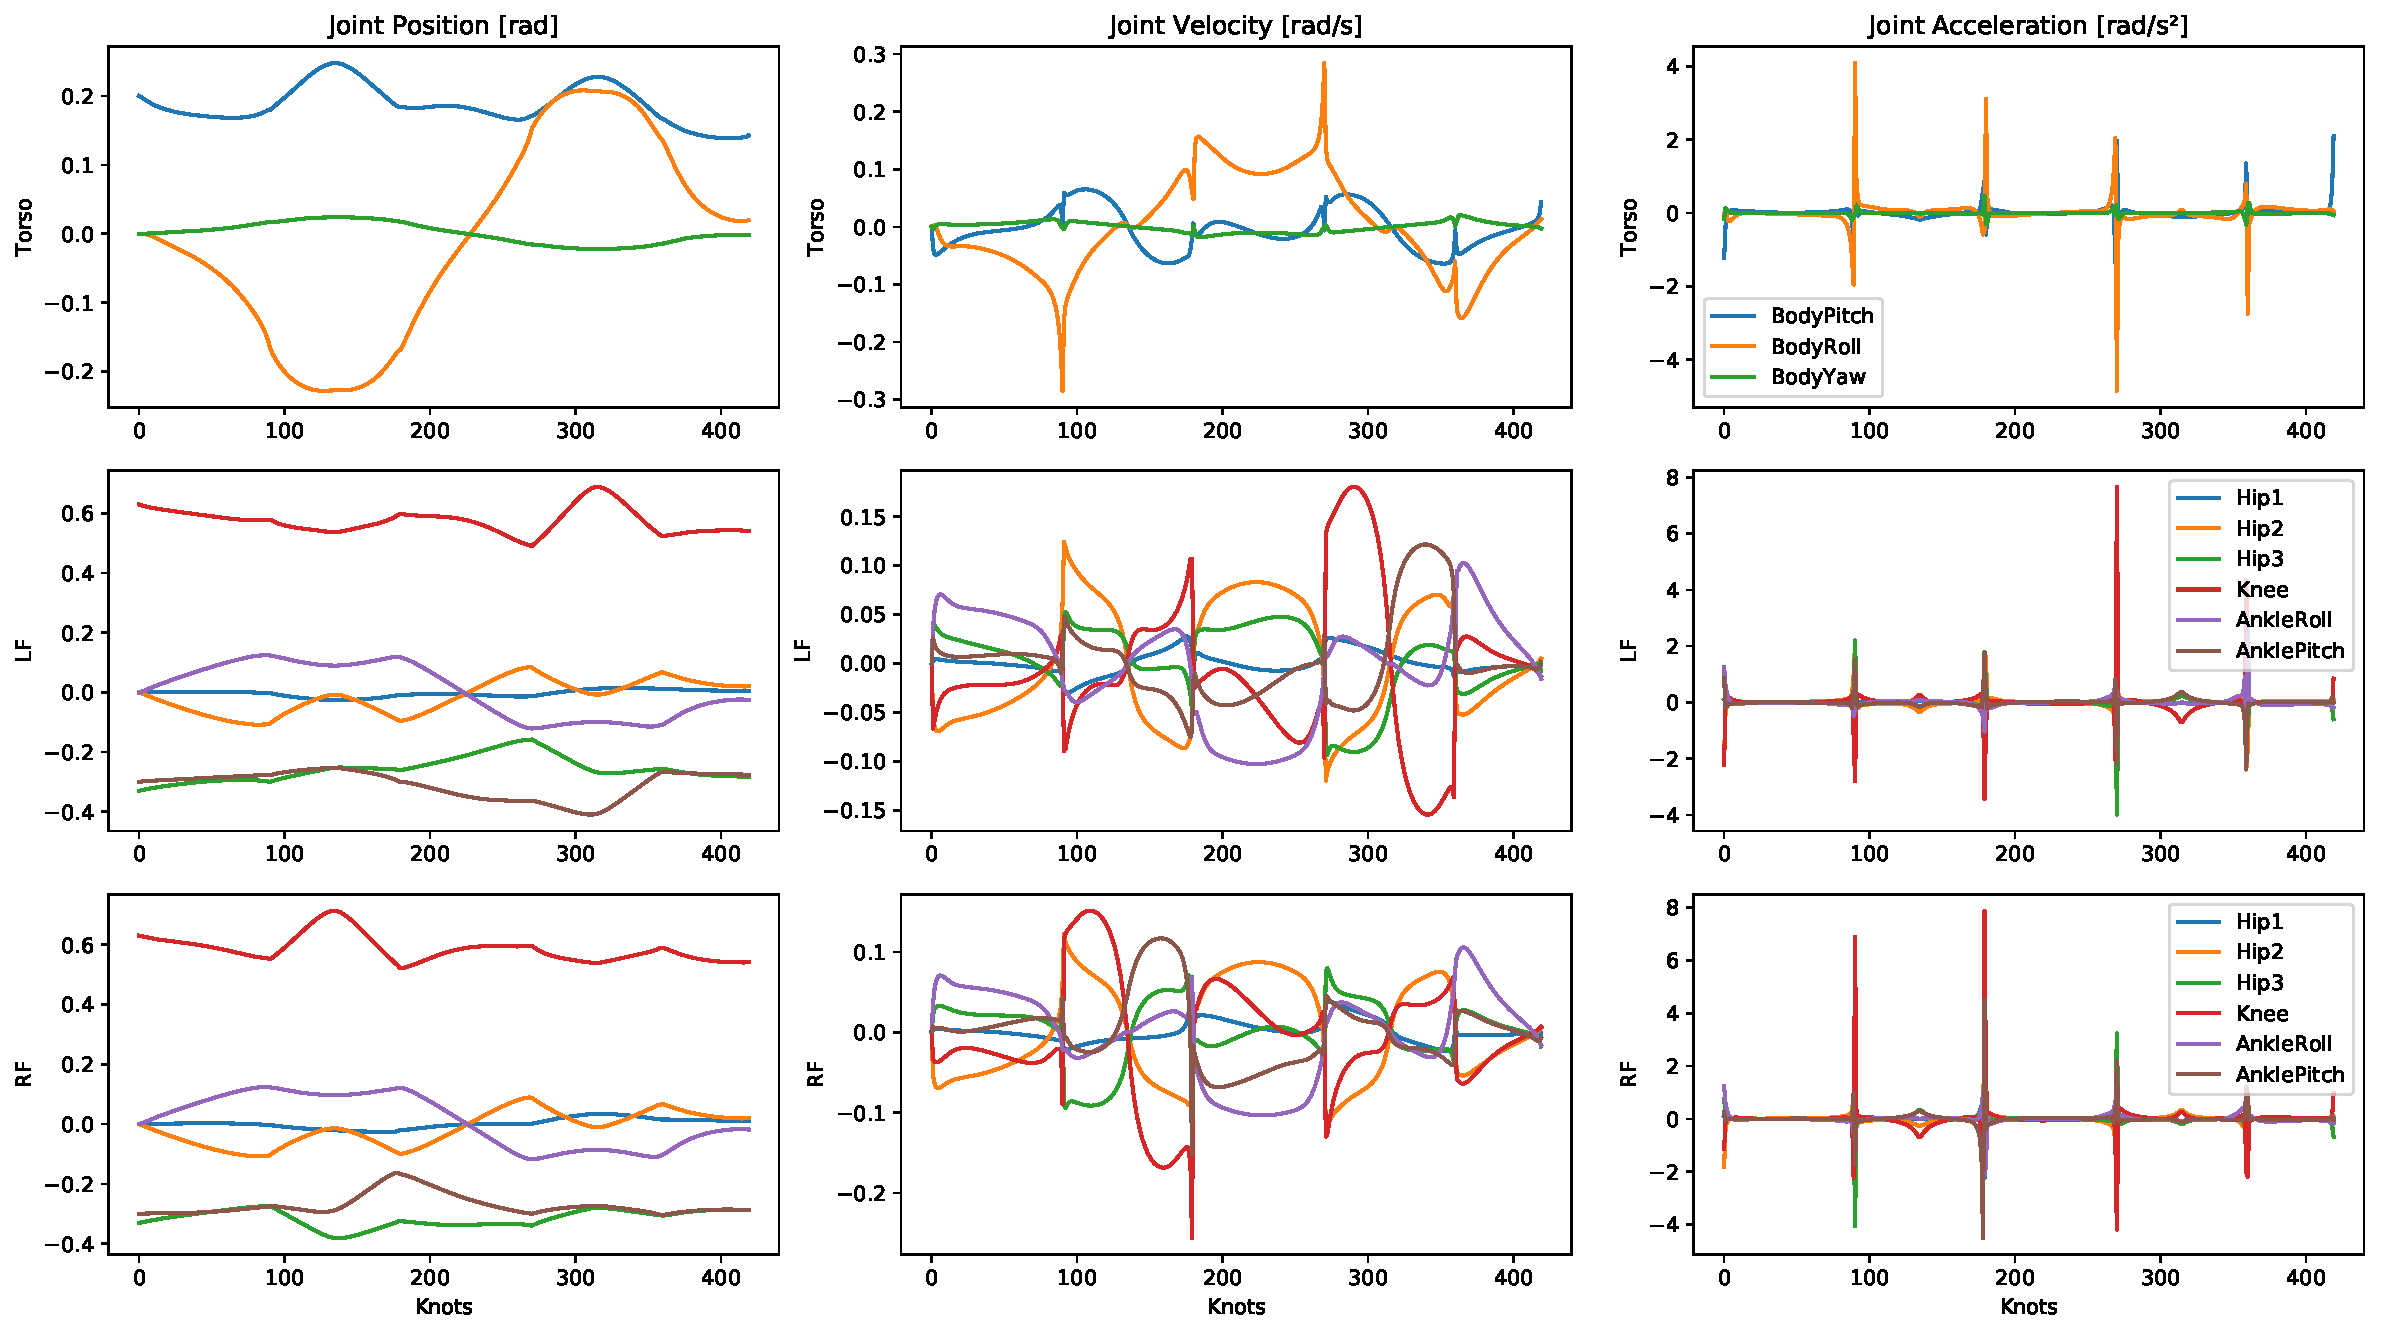
\includegraphics[width=1\textwidth]{fig/walkStatic/JointState}
\caption[Static walking gait solution of the joint states]{Static walking gait solution of the joint states. Due to the slow nature of the motion, joint limits are far from being reached and velocity discontinuities remain within reasonable ranges.}
\label{fig:walkStatic_JointState}
\end{figure} 

\subsection{Dynamic Walking}
The analysis of a dynamic walking gait is concerned about generating efficient motions with higher velocities. This part forms the basis of the stability evaluation in the next section.

Focus of investigation is a dynamic walking motion. Compared to the previously studied static walking gait these motions are characterized by higher velocities and dynamic forces exceeding the static ones. These characteristics imply that dynamic stability criteria become necessary. To this end, we apply the proposed approach of contact stability constrained DDP described in \cref{c3}. Consequently, the \gls{CoP} of each foot is constrained instead of following a reference \gls{CoM} trajectory. By this, the solver is enabled to find an optimal, dynamic \gls{CoM} shifting along with the requested contact stability constraints. 

\cref{tab:walkDynamic} compactly summarizes the gait characteristics and applied optimization constraints. The optimization problem is composed of a total of five locomotion phases visualized in \cref{fig:walkDynamic_Snaps}. From (a) an initial pose in \gls{DS}, (b,c) perform a right step, (d,e) perform a left step and (f) recover to the initial pose. In accordance with biomechanical findings \cite{kuo2001simple}, we choose a desired step length of 40 \nolinebreak cm with 1.5 s per step and deliberately define a stance to swing ratio of one to three.

\begin{table}[t]
\centering
\caption[Dynamic walking gait characteristics and optimization constraints]{Dynamic walking gait characteristics and optimization constraints for a stance to swing ratio of one to three.}
\begin{tabular}{|ll|ll|}
\hline
\multicolumn{2}{|l|}{\textbf{Gait Characteristics}} & \multicolumn{2}{l|}{\textbf{Optimization Constraints}} \\ \hline
Step length:& 40 cm 	& Tasks: 			& $\Phi_{\text{foot}}$\\ \hline
Step height:& 5 cm 	& Stability: 		&$\Phi_{\text{CoP}}$, $\Phi_{\text{friction}}$ \\ \hline
Time:& 1.5 s/step	& Limits: 			& $\Phi_{\text{joint}}$, torques \\ \hline
Step size:& 0.03 s	& Regularization: 	& $\Phi_{\text{posture}}$, $\Phi_{\text{torque}}$\\ \hline
\end{tabular}
\label{tab:walkDynamic}
\end{table} 

\begin{figure}
\begin{subfigure}{.16\textwidth}
	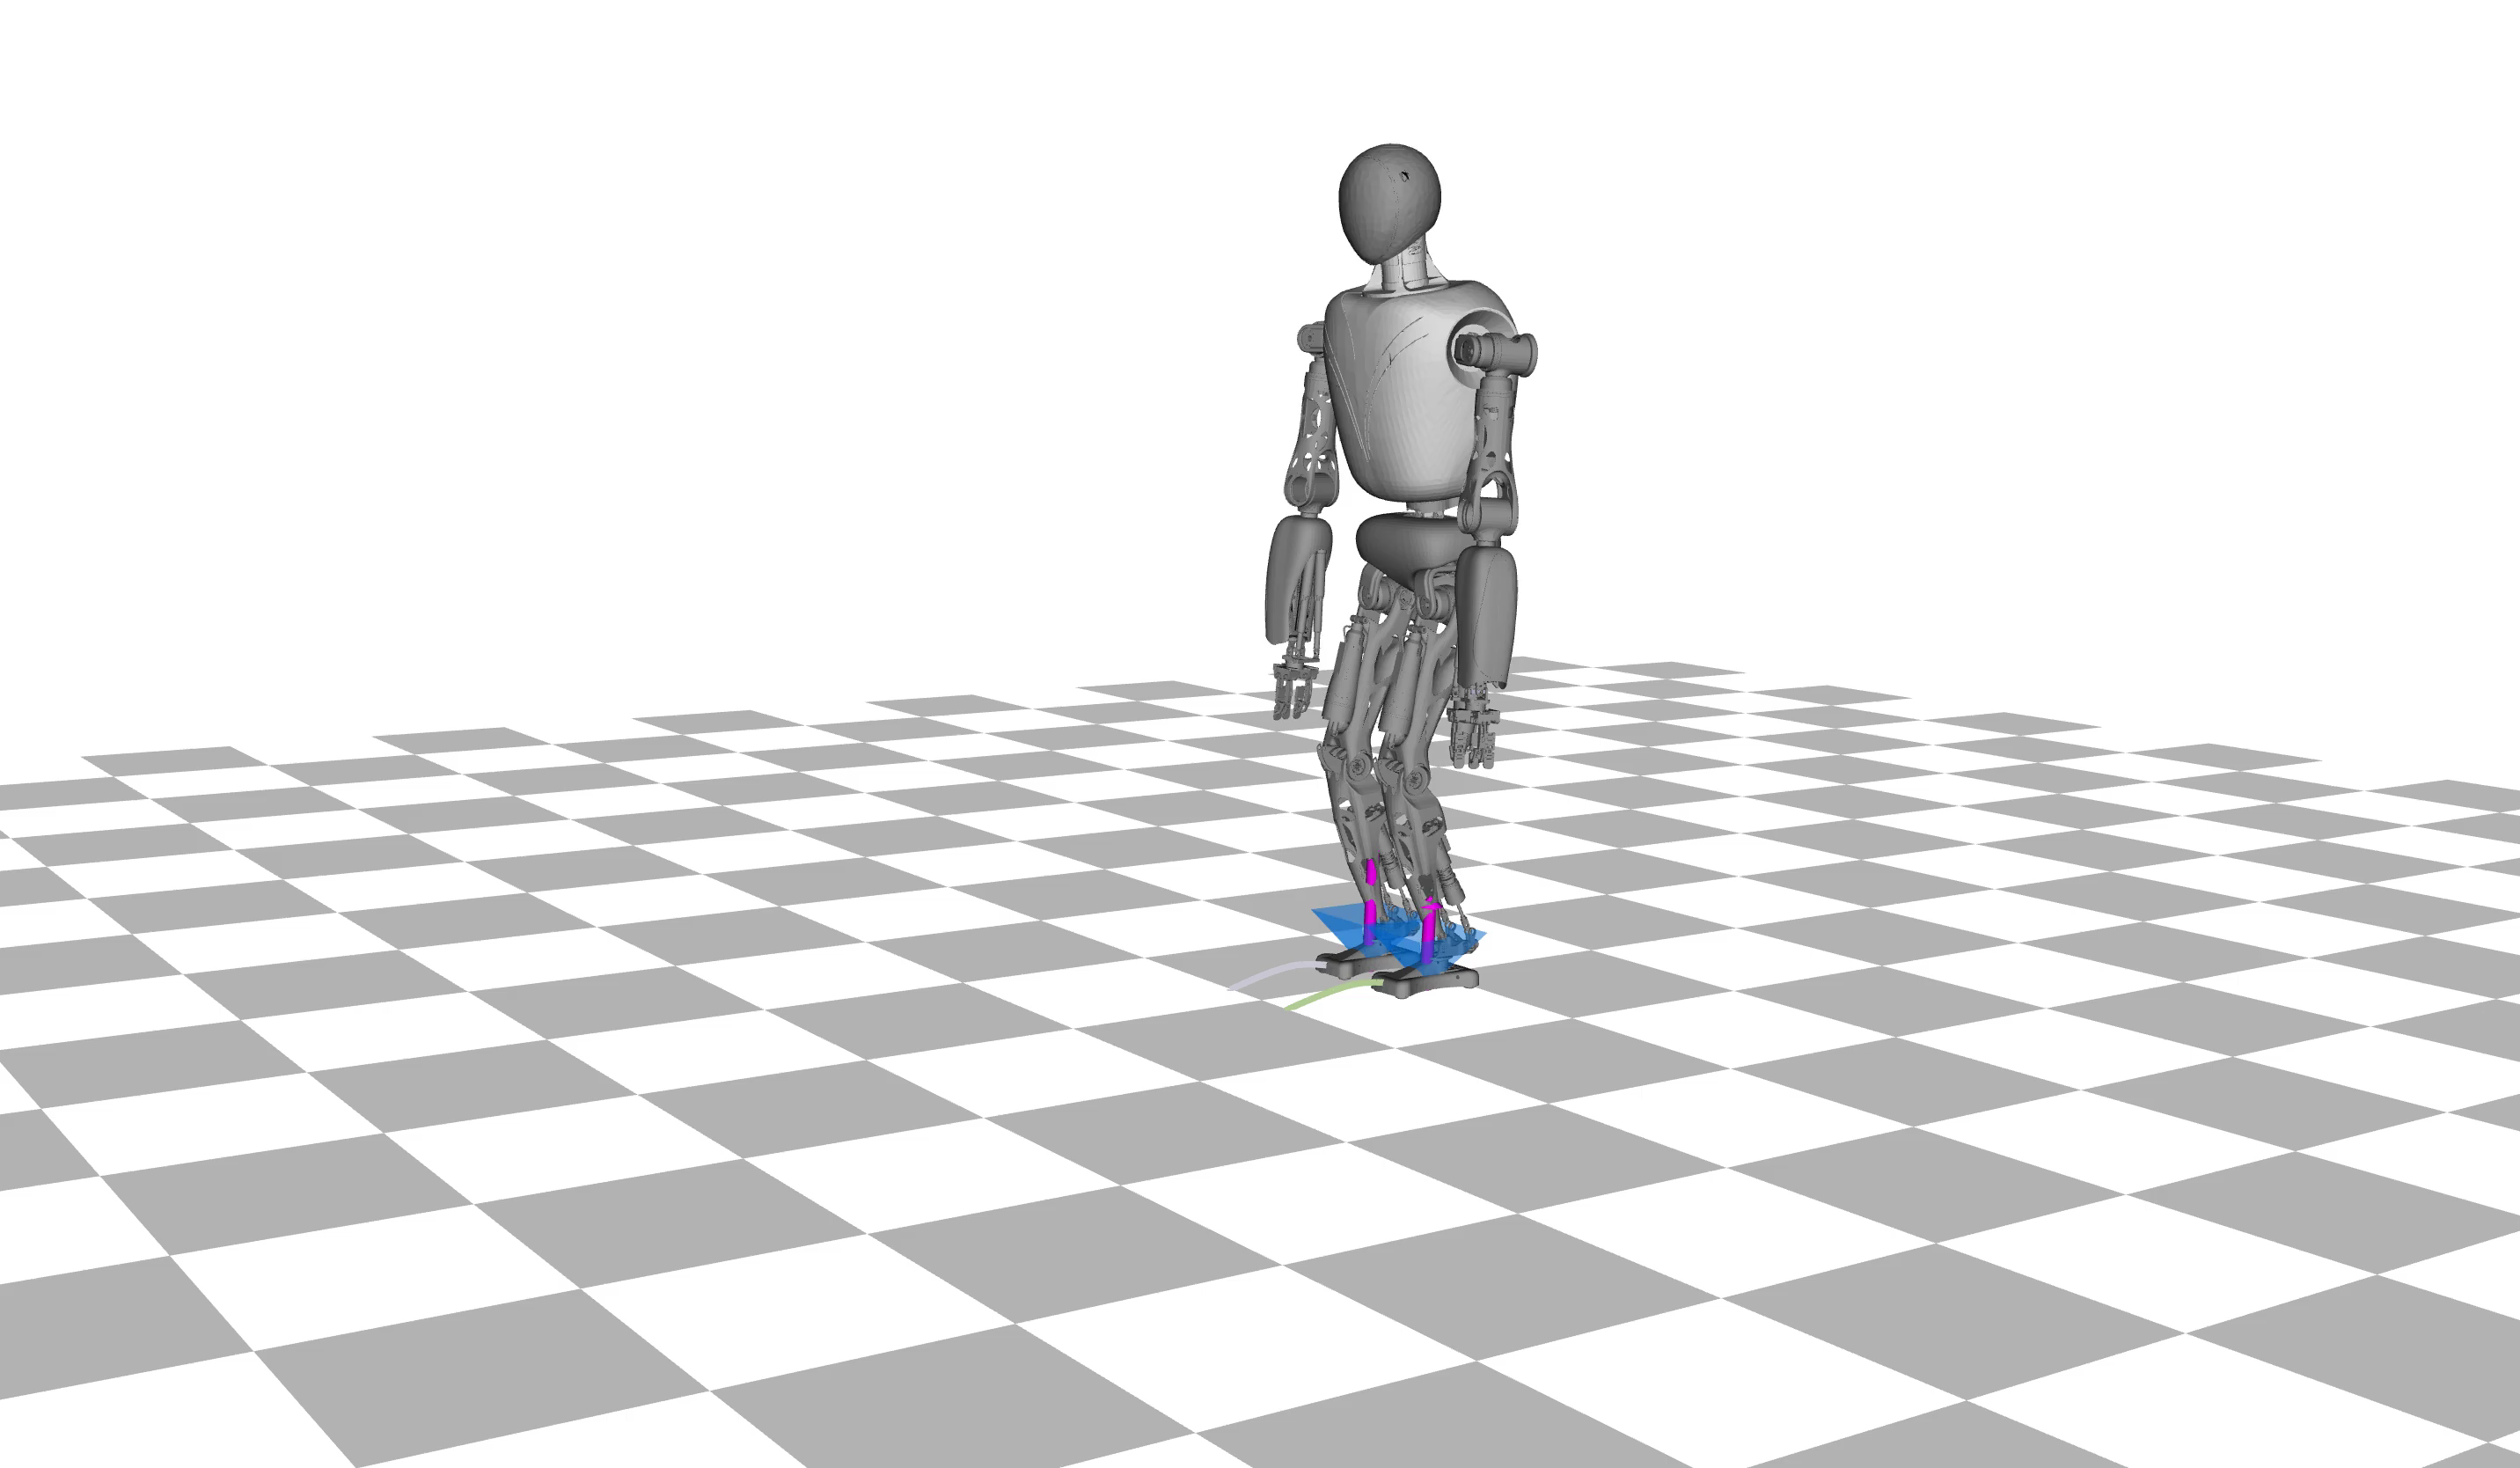
\includegraphics[width=.95\linewidth]{fig/walkDynamic/snaps/1}
	\caption{}
\end{subfigure}%
\begin{subfigure}{.16\textwidth}
	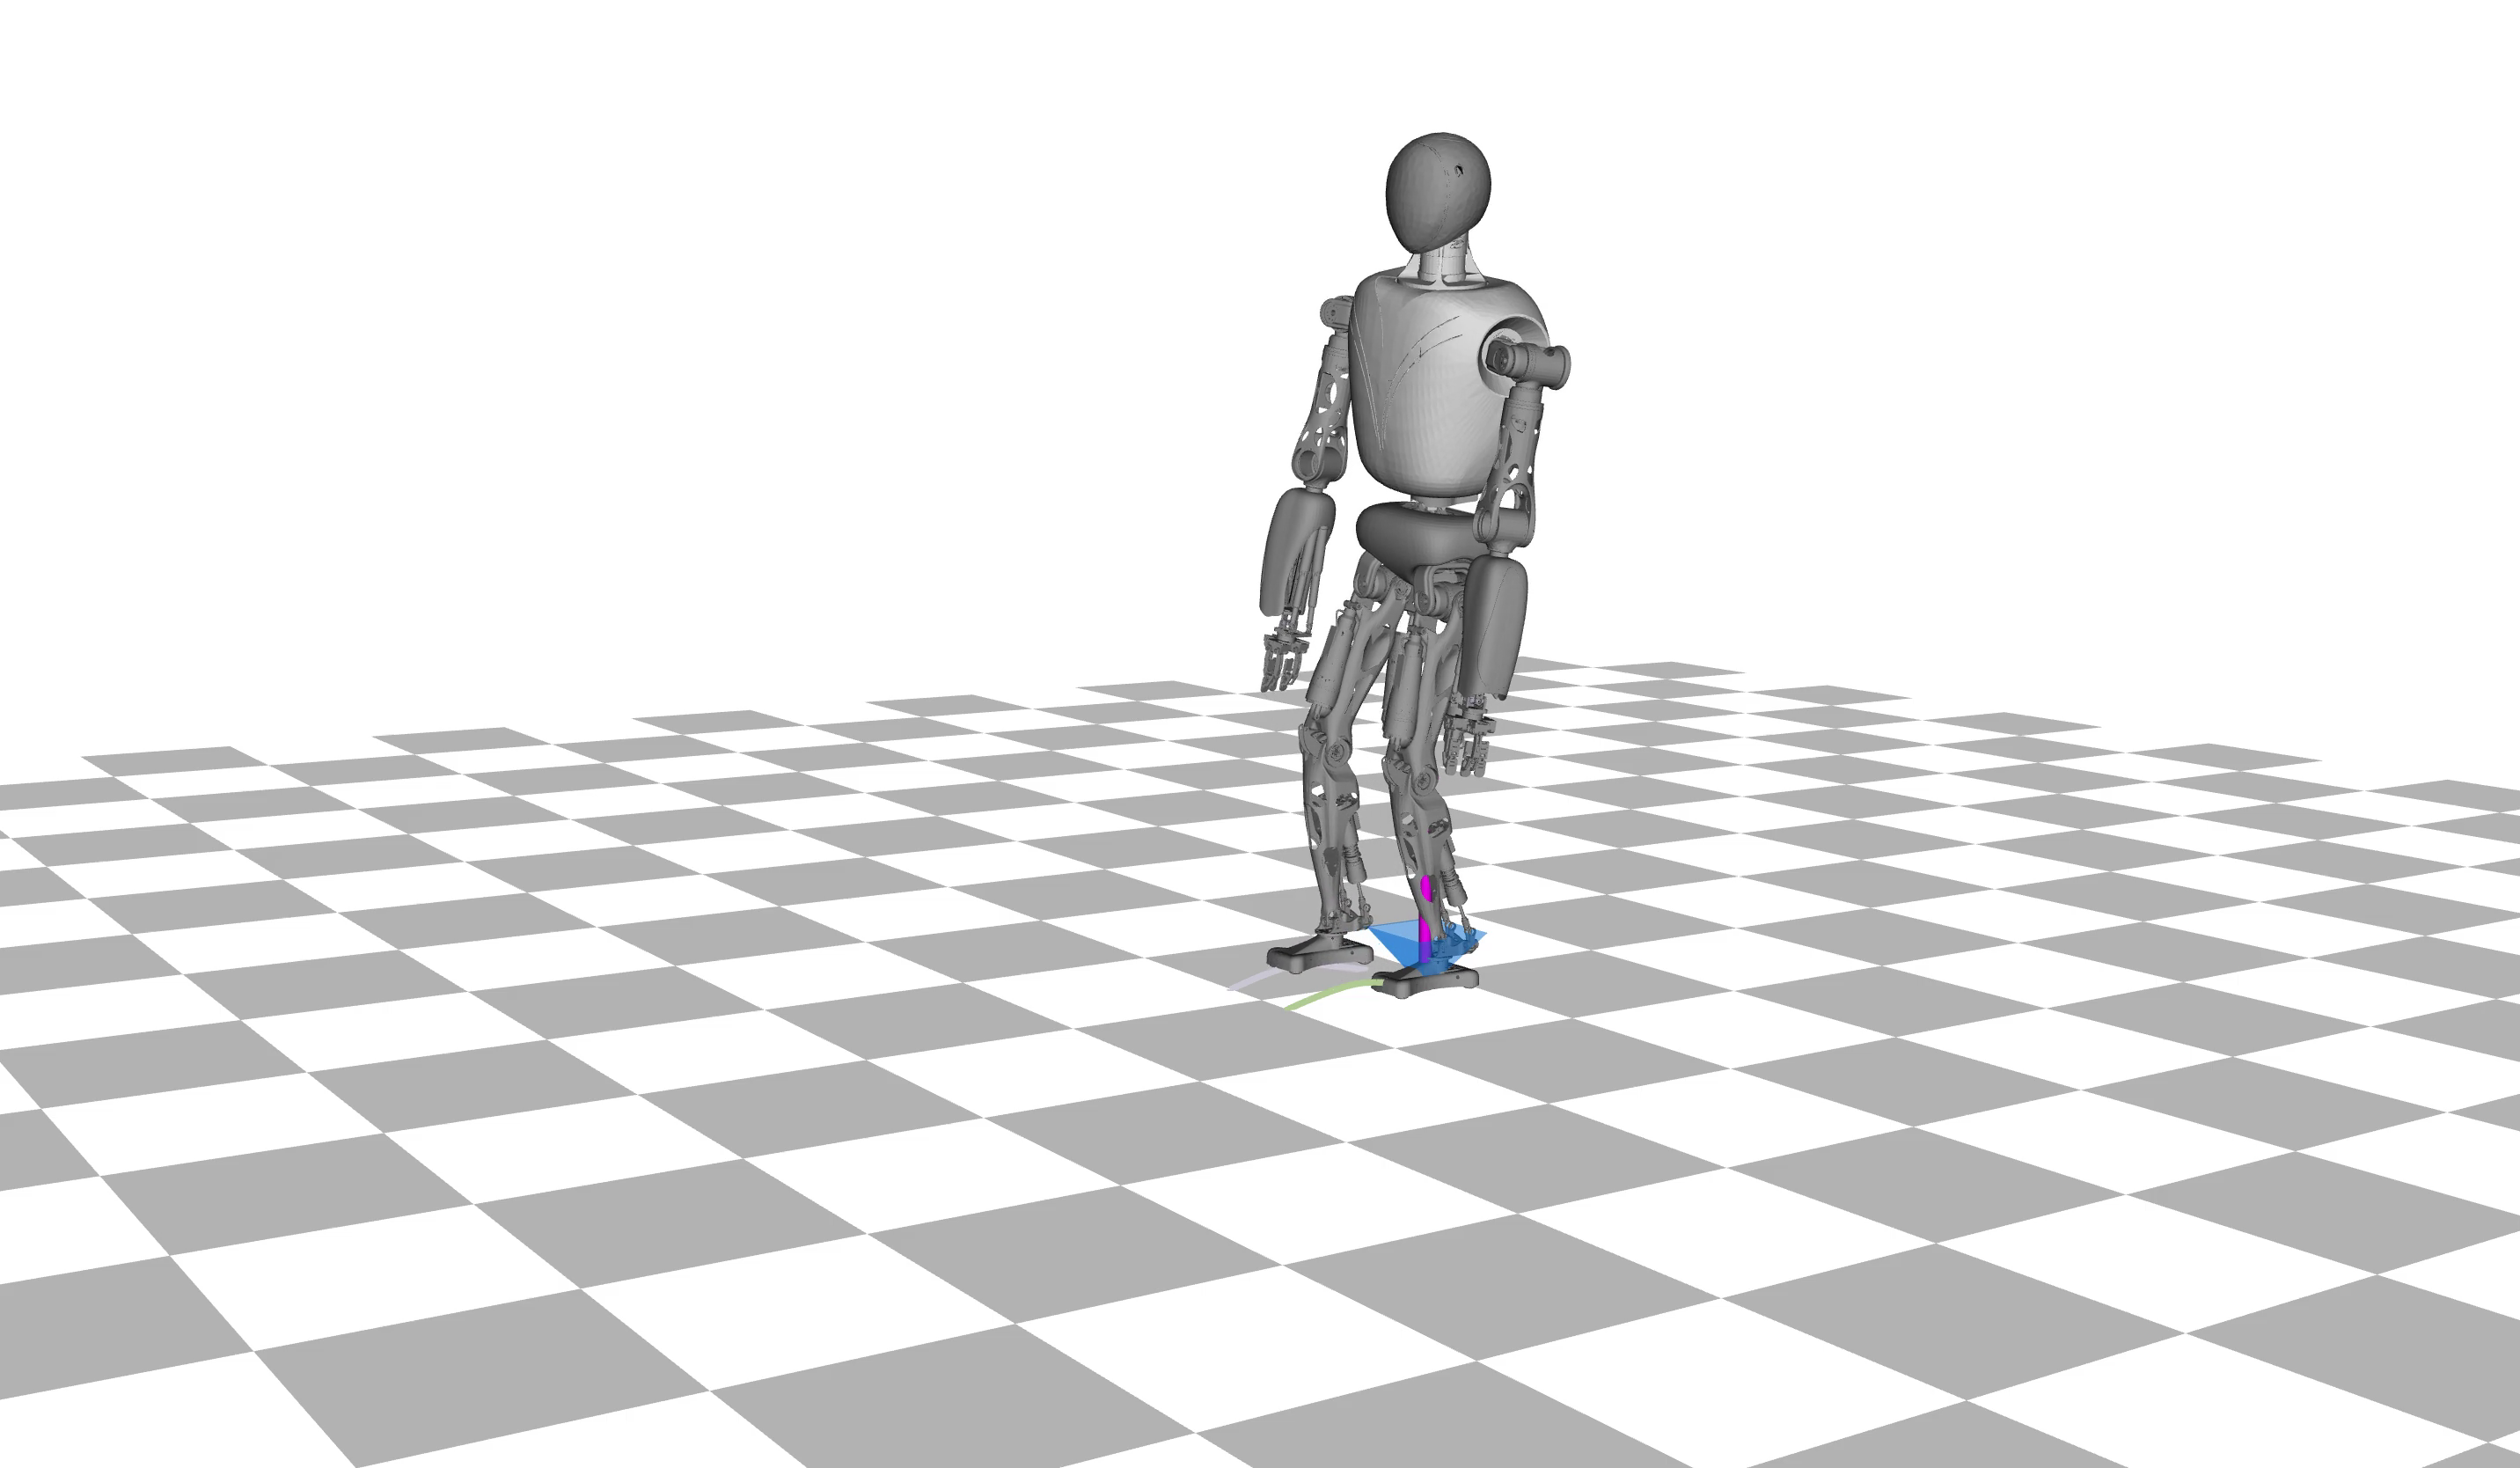
\includegraphics[width=.95\linewidth]{fig/walkDynamic/snaps/3}
	\caption{}
\end{subfigure}%
\begin{subfigure}{.16\textwidth}
	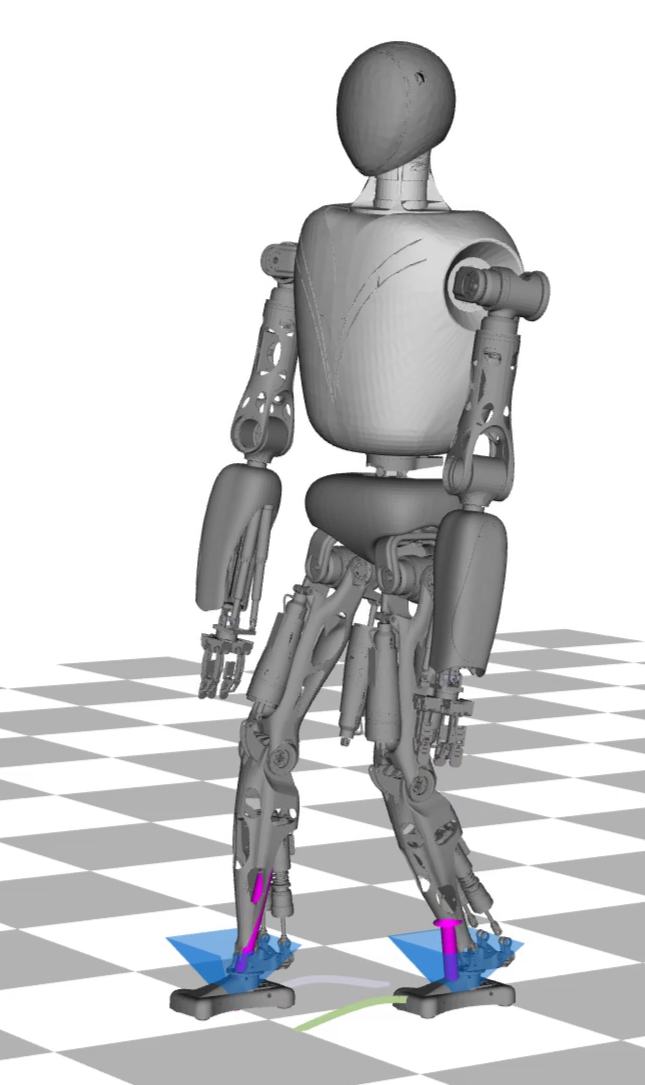
\includegraphics[width=.95\linewidth]{fig/walkDynamic/snaps/4}
	\caption{}
\end{subfigure}%
\begin{subfigure}{.16\textwidth}
	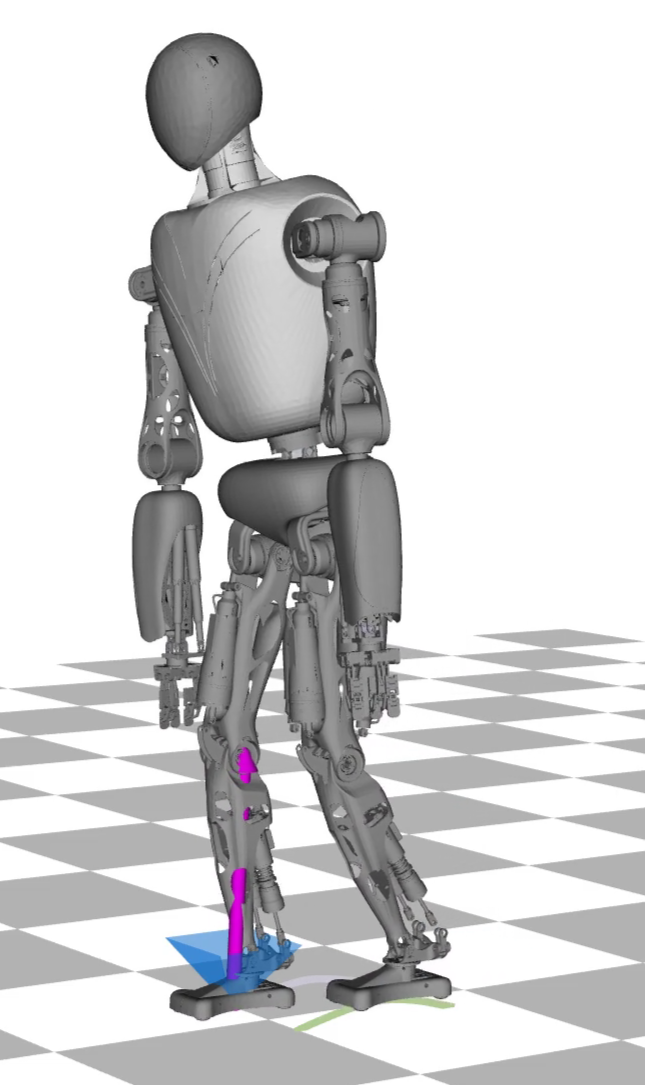
\includegraphics[width=.95\linewidth]{fig/walkDynamic/snaps/6}
	\caption{}
\end{subfigure}%
\begin{subfigure}{.16\textwidth}
	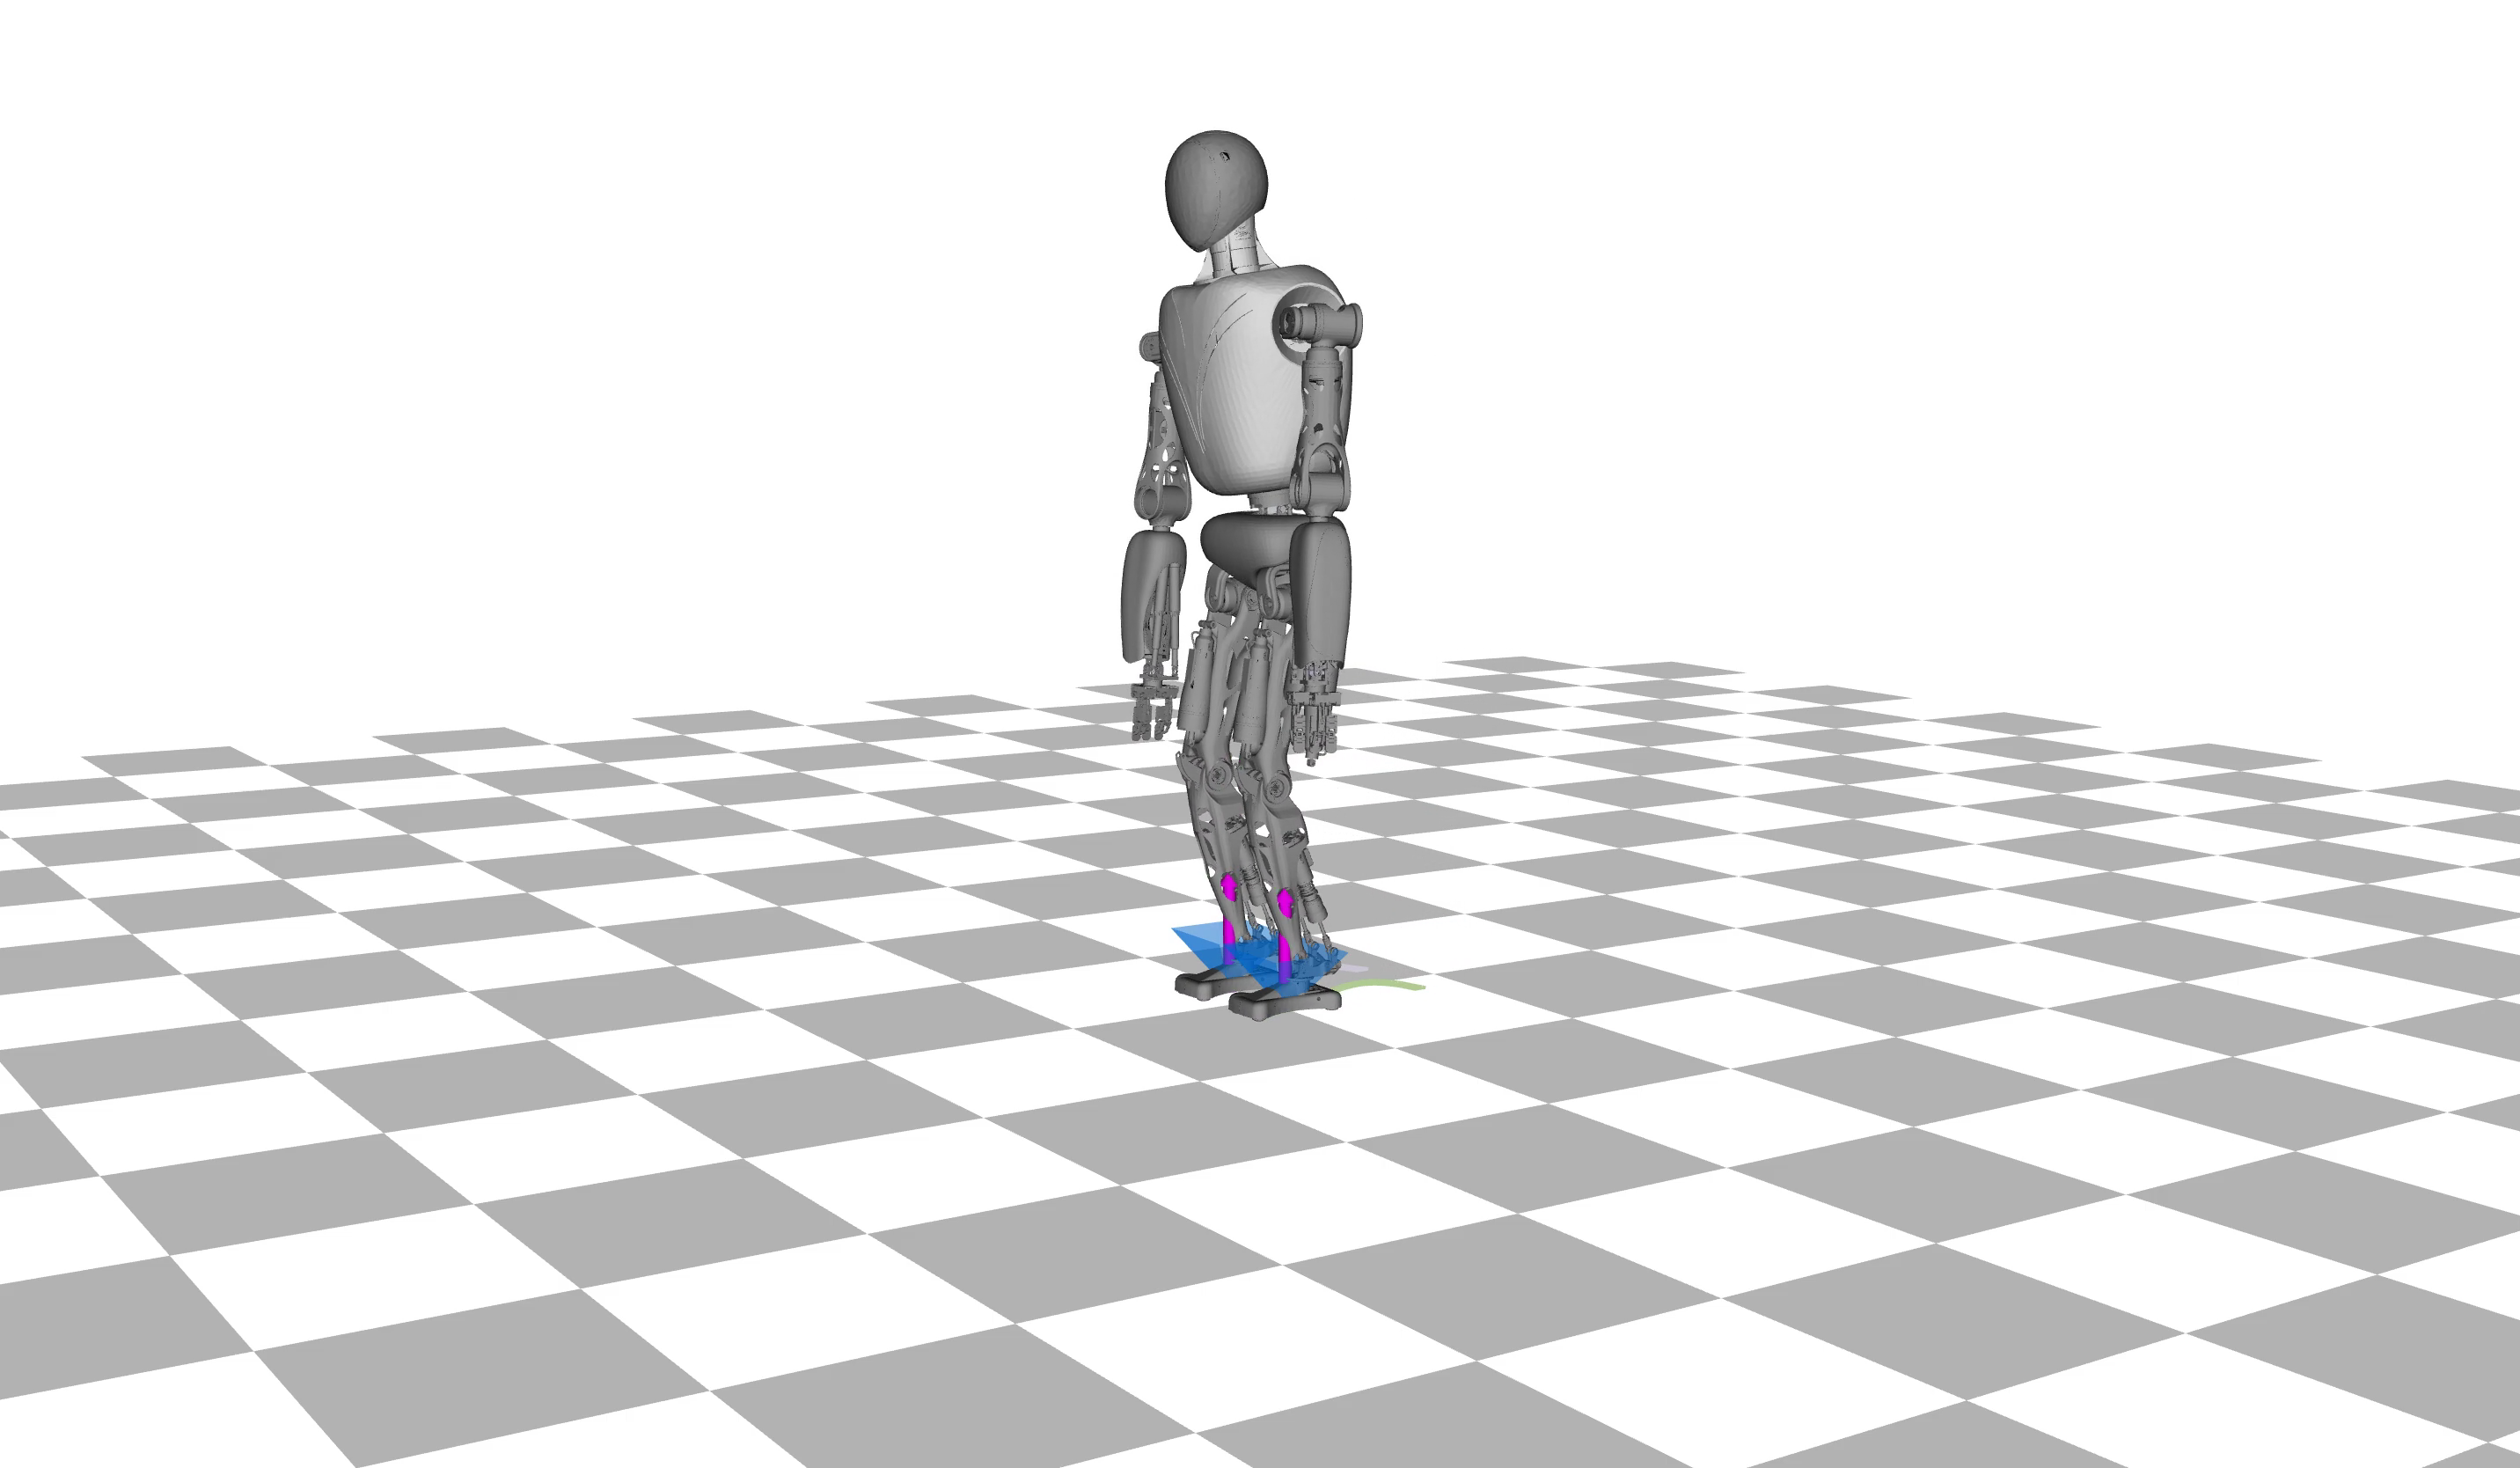
\includegraphics[width=.95\linewidth]{fig/walkDynamic/snaps/7}
	\caption{}
\end{subfigure}%
\begin{subfigure}{.16\textwidth}
	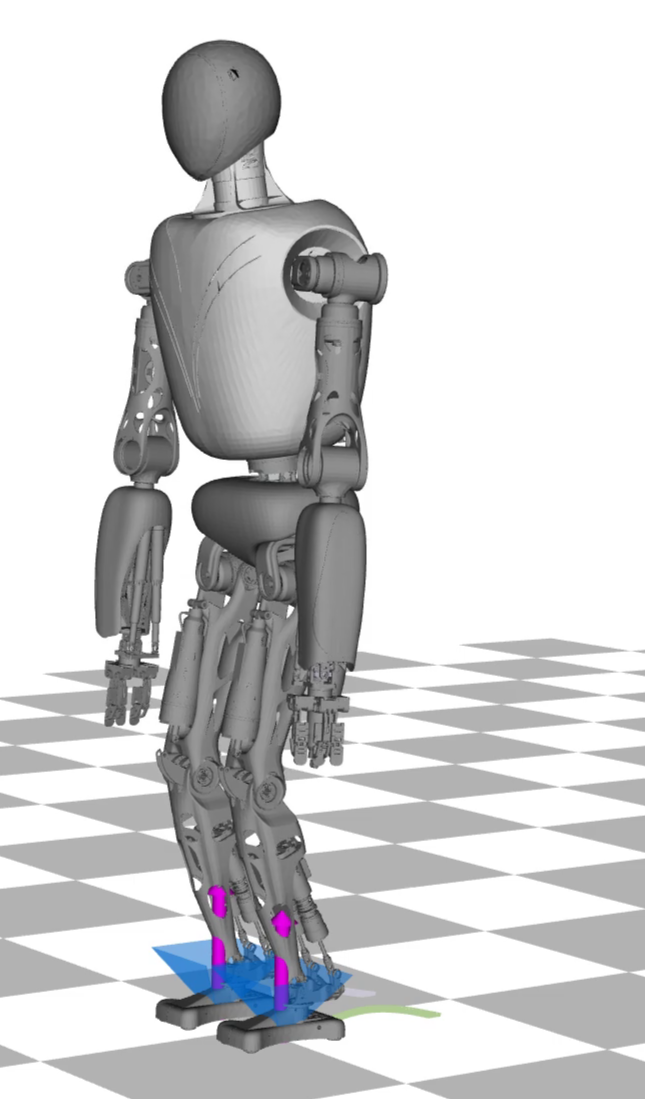
\includegraphics[width=.95\linewidth]{fig/walkDynamic/snaps/8}
	\caption{}
\end{subfigure}
\caption[Dynamic walking based on the contact stability constrained \gls{DDP}]{Dynamic walking gait based on the contact stability constrained \gls{DDP} approach, consisting of the locomotion phases (a) initial pose, (b,c) right step, (d,e) left step and (f) pose recovery. A natural \gls{CoM} shifting emerges resulting from the inequality constraints for the \gls{CoP} of each foot. \href{https://github.com/julesser/ma-thesis-simulation-results/blob/master/DynamicWalking_LargeSteps_CoP100_ArmsFreed/crocoddyl.mp4}{[Video]}}
\label{fig:walkDynamic_Snaps}
\end{figure}

As becomes clear from \cref{fig:walkDynamic_TaskSpace}, a natural \gls{CoM} shifting to the sides emerges resulting from the inequality constraints for the \gls{CoP}, which is about half of the amount as for the static walking case. Although the \gls{CoM} height is not explicitly constrained, it stays in a reasonable range of about $+$3 cm, which may be caused from the final posture regularization. The end-effector velocities in z-direction are about twice as high as for the case of static walking, which is explained by the higher walking speed. 
\cref{fig:walkDynamic_JointState} shows the resulting joint states for the dynamic walking gait. The velocity and acceleration contain higher peaks and the joint deflections are stronger, which is reasonable due to the higher walking speed.       

\begin{figure}[h!]
\centering	
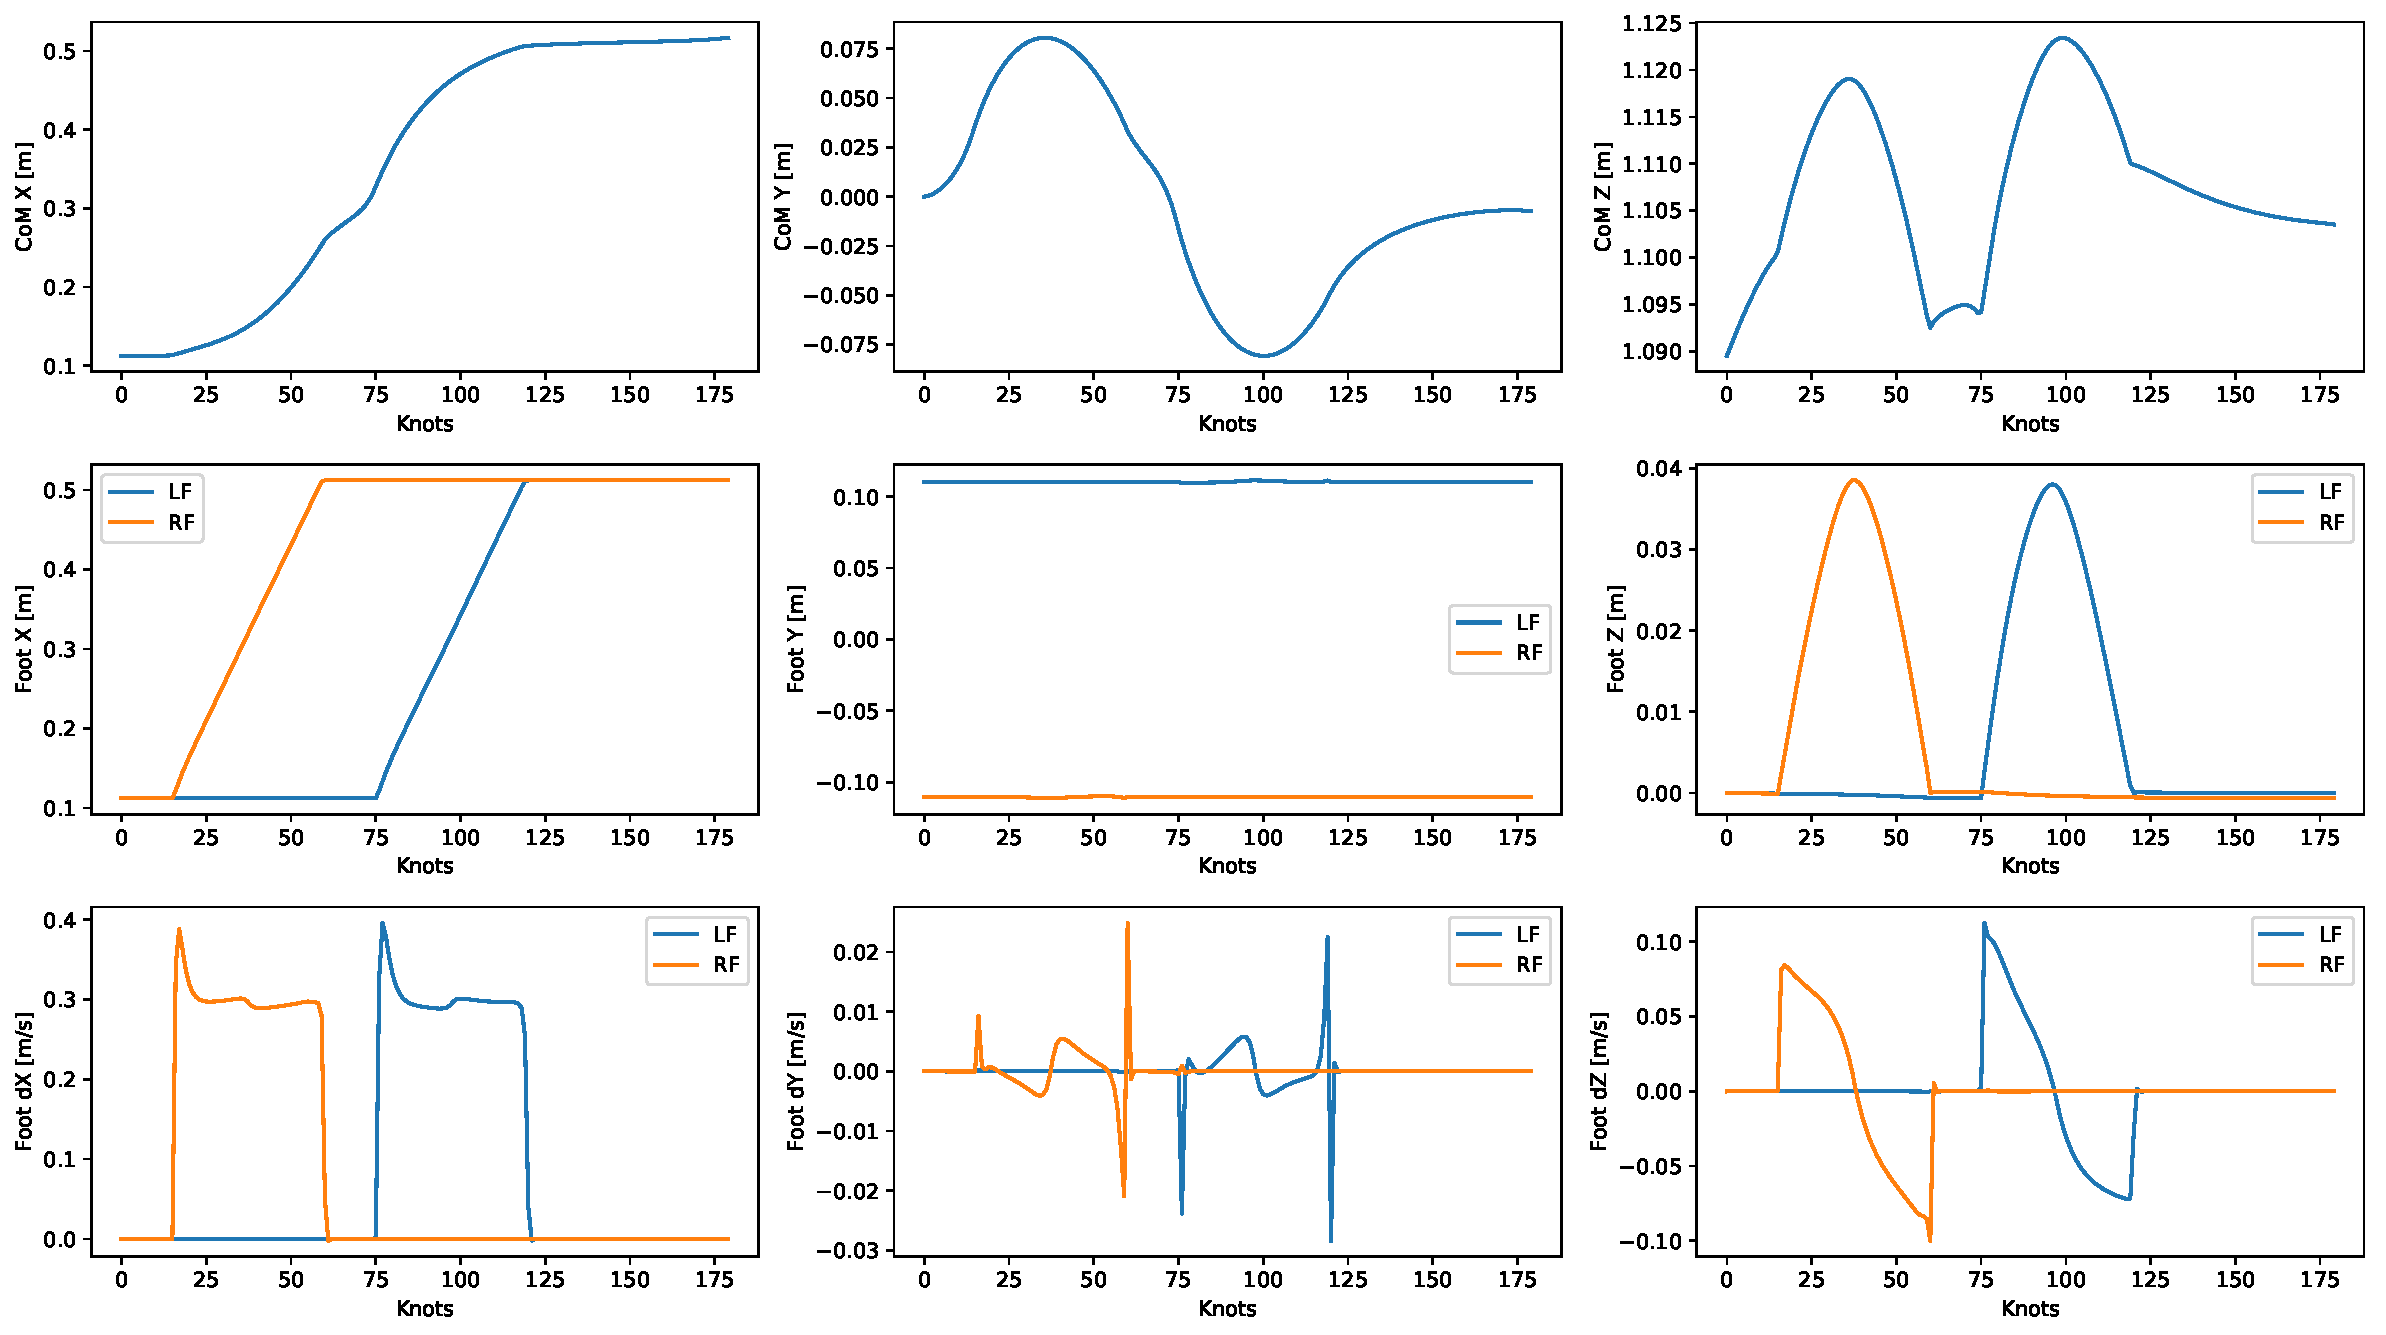
\includegraphics[width=.9\textwidth]{fig/walkDynamic/TaskSpace}
\caption[Dynamic walking gait solution in task space]{Dynamic walking gait solution in task space. It becomes evident that a natural \gls{CoM} shifting in y-direction emerges resulting from the inequality constraints for the \gls{CoP} of each foot.}
\label{fig:walkDynamic_TaskSpace}
\end{figure} 

\begin{figure}[h!]
\centering	
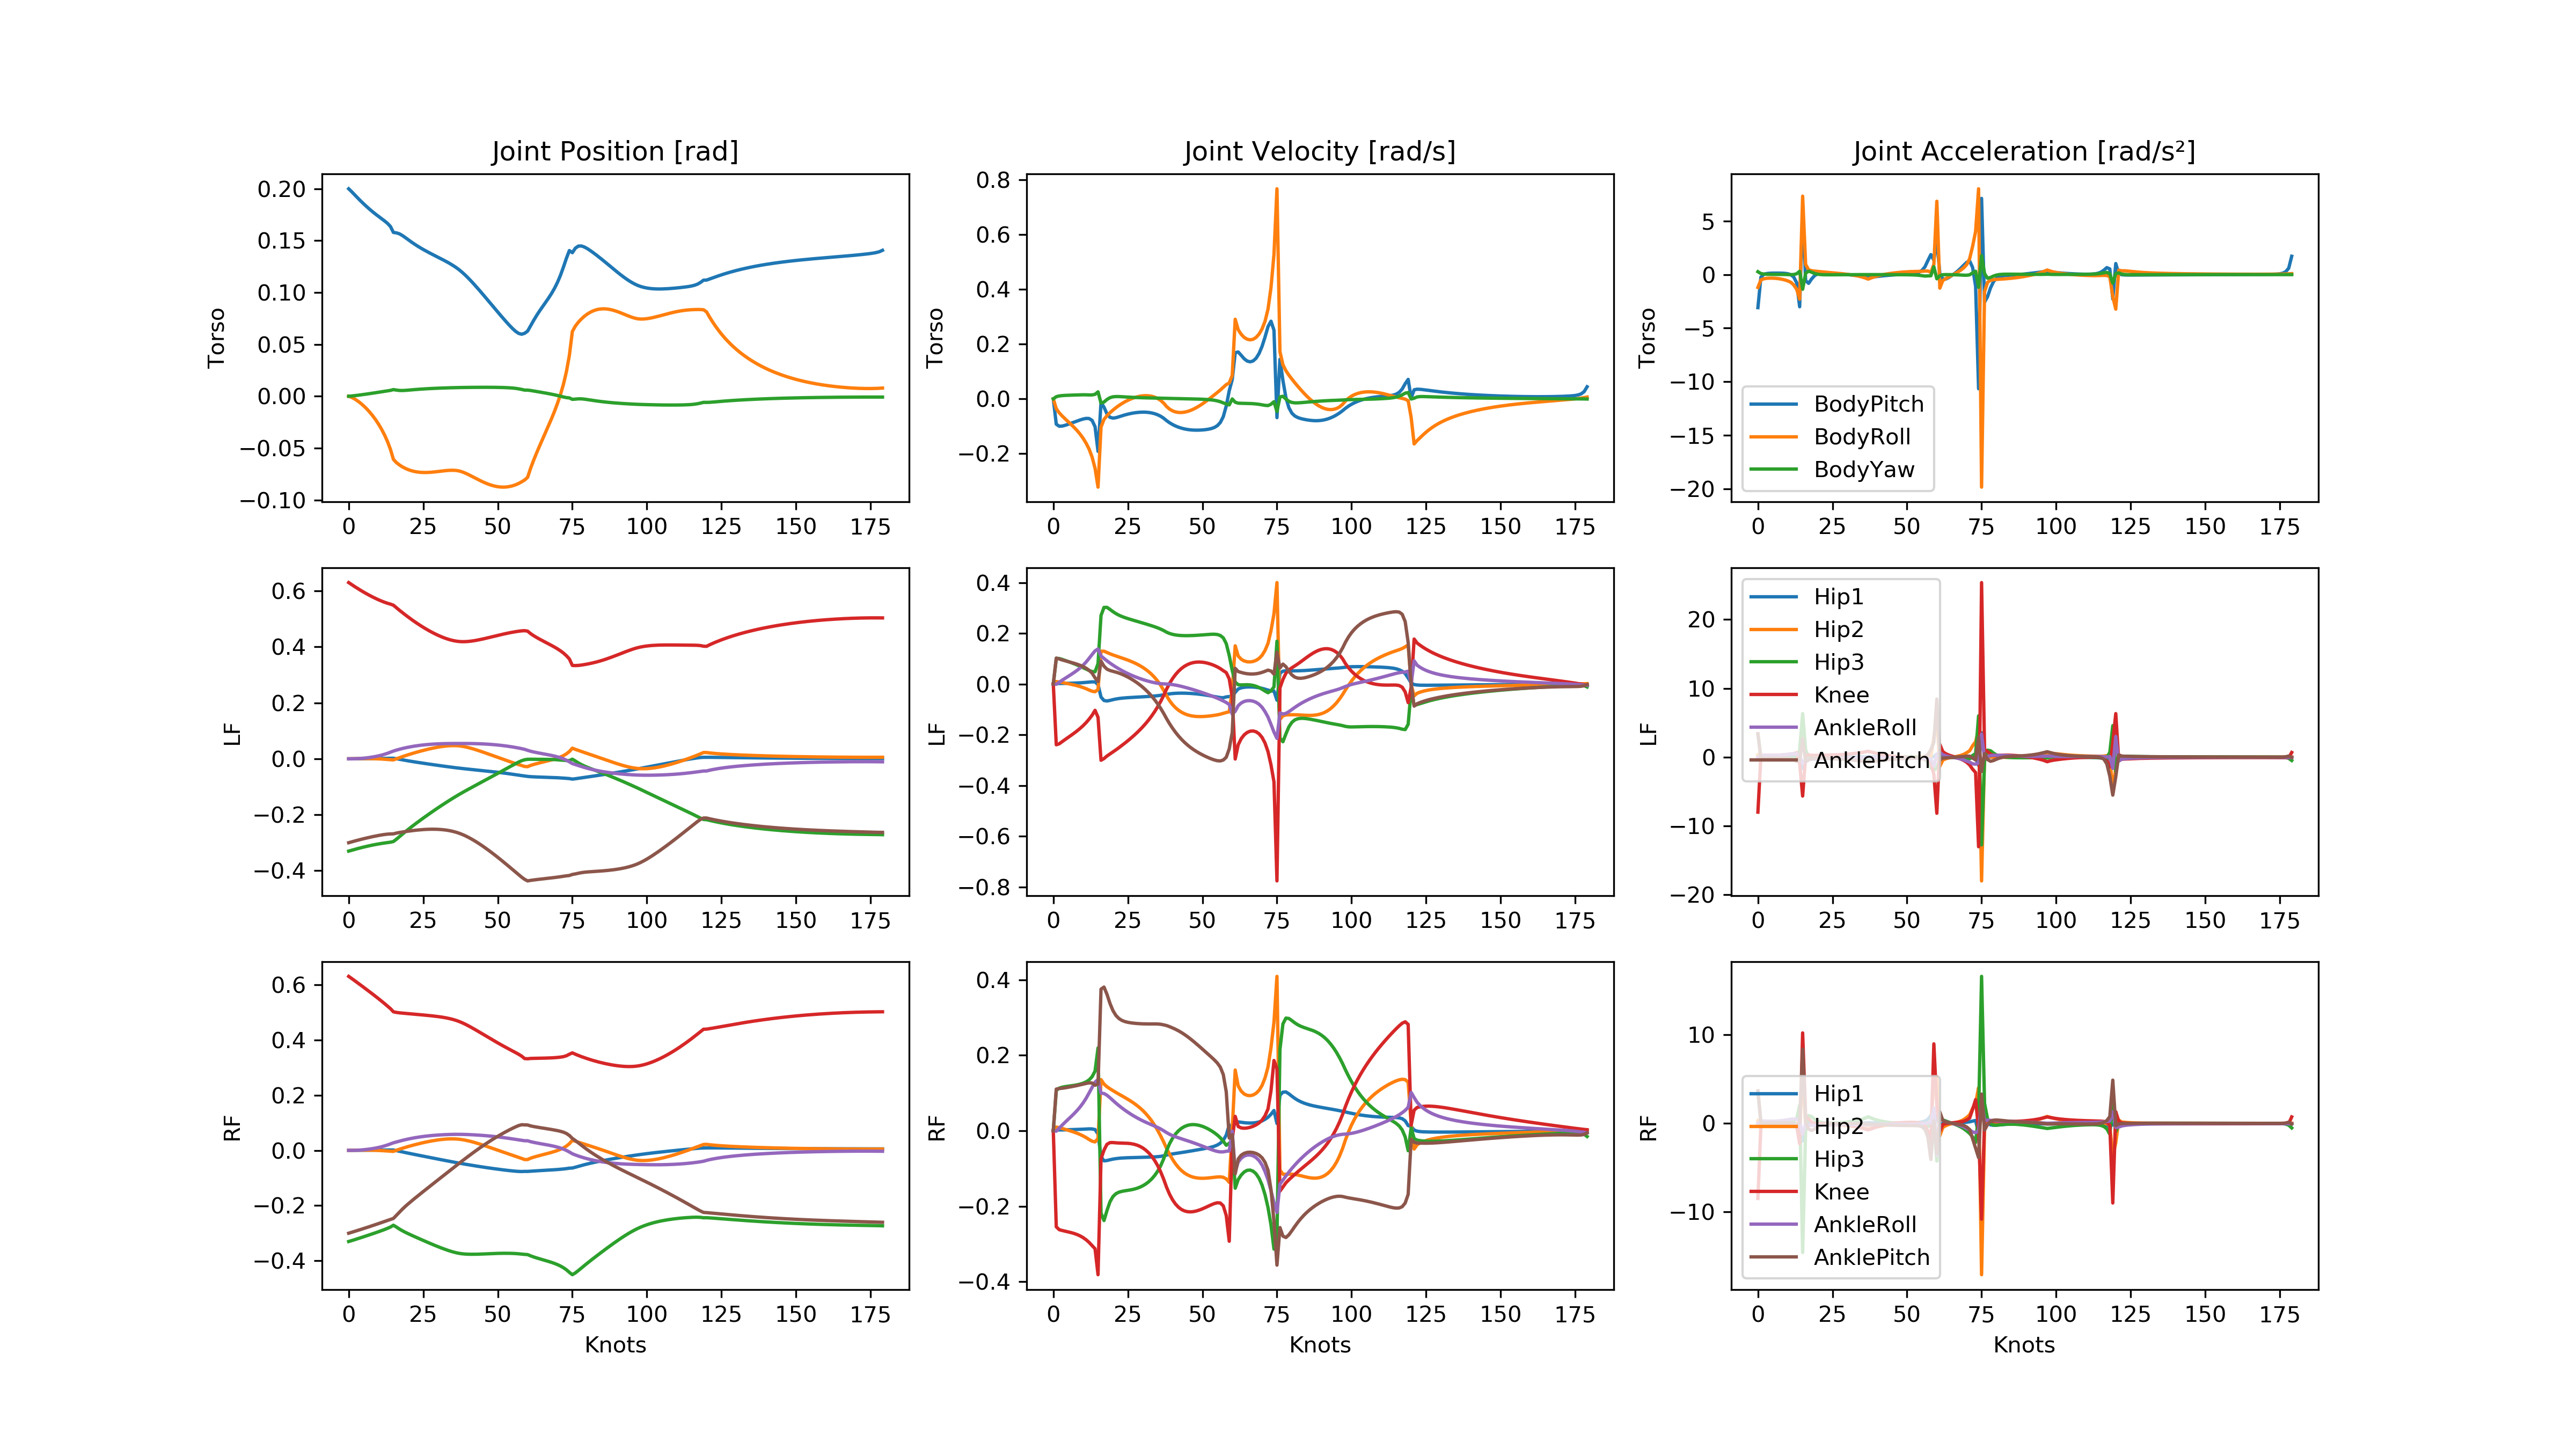
\includegraphics[width=.9\textwidth]{fig/walkDynamic/JointState}
\caption[Dynamic walking gait solution of the joint states.]{Dynamic walking gait solution of the joint states. Both joint velocities and acceleration show higher peaks along with higher joint deflections compared to the static walking, which is reasonable due to the higher walking speed.}
\label{fig:walkDynamic_JointState}
\end{figure} 

%\subsection{Dynamic Walking: Long Gait as Sequence of OC Problems}
%\subsection{Dynamic Walking: The Effect of Different Velocities}


\section{Evaluation of Contact Stability}\label{sec:BipedEvaluation}
This section evaluates, based on the presented dynamic walking gait from the previous section, the proposed approach of contact stability constrained DDP (\cref{c3}).

\subsection{Dynamically Balanced Walking Motion}
As detailed in \cref{sec:TheoryStability}, the central characteristic for dynamically balanced motions is that the \gls{CoP} or \gls{ZMP} remains within the \gls{SP}. The generic approach presented in \cref{c3} has been applied to the dynamic walking gait presented in the previous section. It utilizes the \gls{CoP} criterion for each contact surface and hence the motion can be called dynamically balanced only if the \gls{CoP} of each foot in contact stays within the according \gls{SP} along the whole motion. 

\cref{fig:walkDynamic_StabilityCoP100} shows the top view of the presented dynamic walking  gait. The rectangles correspond to the true-to-scale dimensions of the robot feet. For clarity, only the first and last \gls{DS} phase are visualized.  
The blue curve shows the time course of the resulting \gls{CoM} trajectory, with relevant points in time marked separately. Since the \gls{CoM} trajectory between lift-off and touch-down is largely outside the respective foot area, no static stability can be present, as expected. 
The orange and green crosses mark the time-dependent position of the \gls{CoP}s for both feet. It is evident that both \gls{CoP}s remain within the corresponding SP over the entire time course of the movement, which is why the movement can be classified as dynamically balanced. 

\subsection{Different Levels of CoP Restriction}
Although the dynamic walking motion is inherently balanced, it becomes clear from \cref{fig:walkDynamic_StabilityCoP100} that the \gls{CoP} partly lies \textit{on} or \textit{near} the border of the respective foot area. This effect can be attributed to the formulation of the \gls{CoP} cost function (\cref{eqn:CoPCostComputation}), which is defined to be zero whenever the \gls{CoP} lies within the given foot area and a quadratic penalization prevents the \gls{CoP} to leave the \gls{SP}. 
Theoretically, this formulation is sufficient to generate balanced motions. 
In practice however, it might be convenient for real-world experiments to consider a dedicated safety factor so that the \gls{CoP}s maintain a certain distance from the edge. With the presented \gls{CoP} cost function, this objective can be easily achieved by reducing the desired foot geometry. 
\cref{fig:walkDynamic_StabilityCoP50} shows the dynamic walking gait, where the \gls{CoP} inequality constraints are active for a \gls{SP} reduced to 50 percent of the original foot geometry. It becomes evident that also these more conservative contact stability constraints can be solved, which might be useful for the purpose of experimental validation. 

\begin{figure}[h!]
\centering	
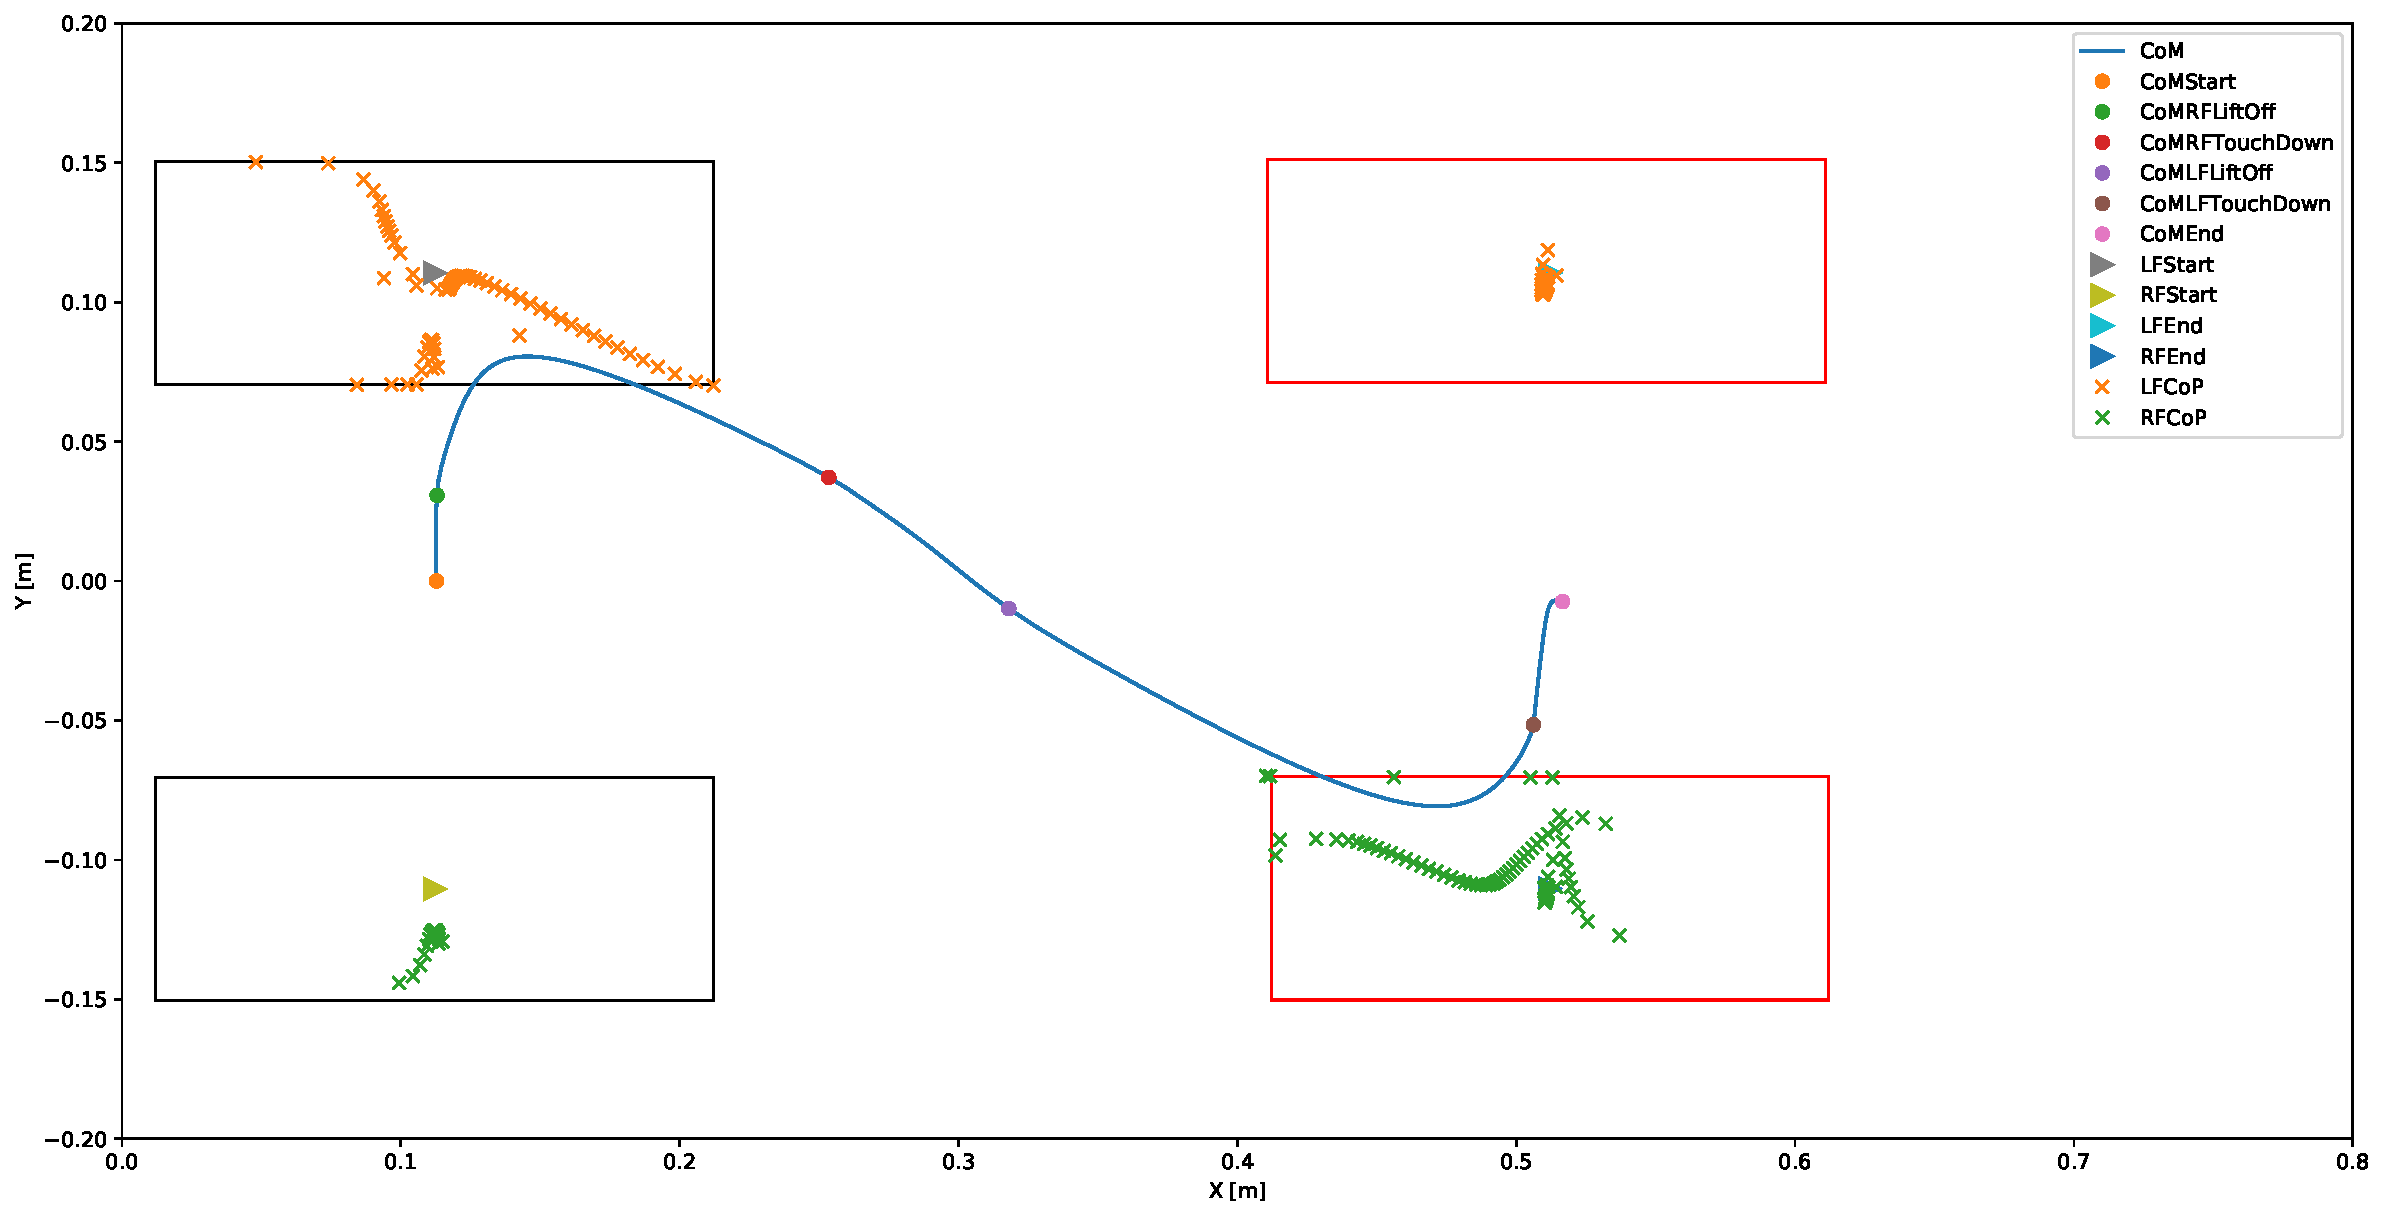
\includegraphics[width=1\textwidth]{fig/walkDynamic/StabilityAnalysis_CoP100}
\caption[Stability Analysis of the dynamic walking gait]{Stability Analysis of the dynamic walking gait. As both \gls{CoP}s remain within the corresponding SP, the movement can be classified as dynamically balanced. Hence, the functionality of the proposed contact stability constrained \gls{DDP} approach is verified.}
\label{fig:walkDynamic_StabilityCoP100}
\end{figure} 

\begin{figure}[h!]
\centering	
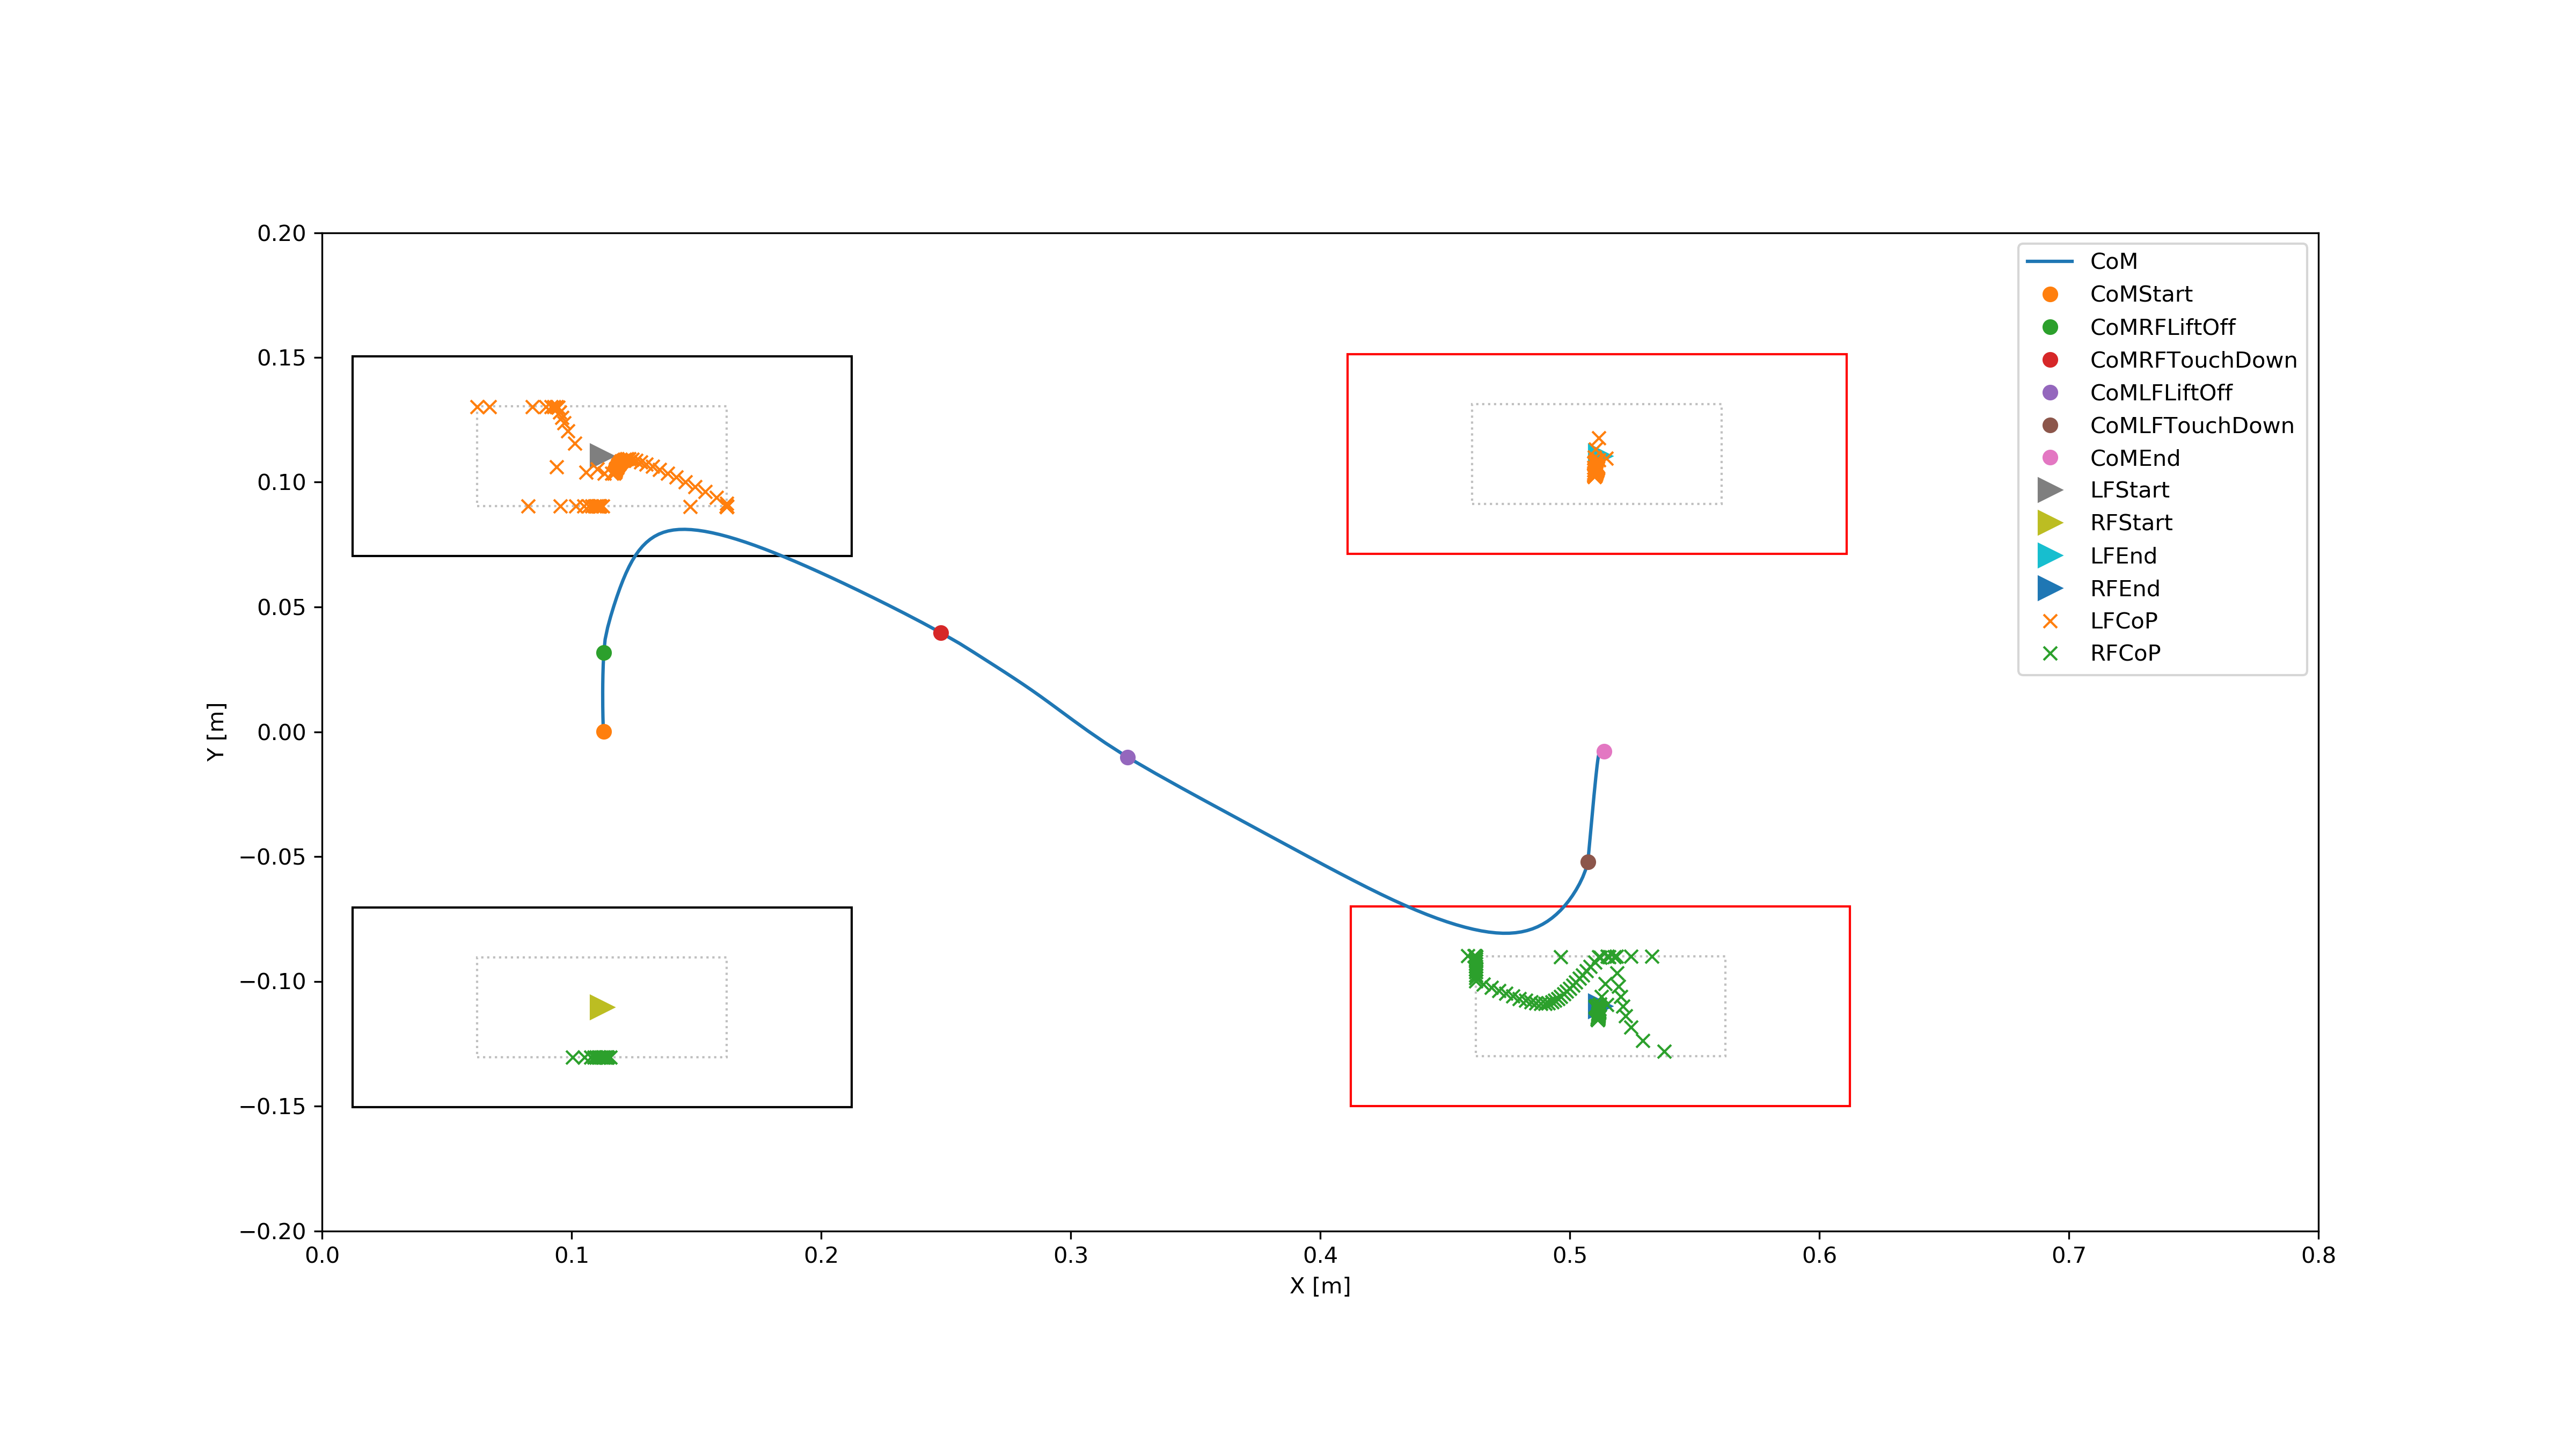
\includegraphics[width=1\textwidth]{fig/walkDynamic/StabilityAnalysis_CoP50}
\caption[Dynamic walking stability analysis with conservative \gls{CoP} restriction]{Stability analysis of the dynamic walking gait with a \gls{CoP} that is constrained in a \gls{SP} reduced by 50 percent. By this, the stability is more conservative, which may be convenient for real-world experiments}
\label{fig:walkDynamic_StabilityCoP50}
\end{figure}

In this section we have seen that the proposed contact stability constrained DDP produces motions that are dynamically balanced. In \cref{c6} we investigate if the generated motions can be tracked by a simple online stabilizer based on position control in joint space. Beforehand, in \cref{c5}, we explore the effect of the motion planning approach and physical system limits on highly dynamic movements.
























